\documentclass[12pt]{amsart}
\usepackage{tikz-cd}
%\usepackage{enumitem}
%\setlist[description]{leftmargin=\parindent,labelindent=\parindent}
\usepackage{amssymb}
\usepackage{amsmath,amscd}
\usepackage{mathrsfs}
\usepackage{mathtools}
\usepackage{url}
\usepackage{cite}
\usepackage{fullpage}
\usepackage[hidelinks]{hyperref}
\usepackage{verbatim}
\usepackage{comment}
\usepackage{fancyvrb}
\usepackage{fvextra}
\usepackage{caption}
\usepackage{tikz}
\usepackage{tkz-graph}
\usetikzlibrary{matrix}
 \usetikzlibrary{shapes}
\usetikzlibrary{arrows,decorations.markings}
\usepackage{tikz-cd}
\usepackage{stmaryrd}

\pgfarrowsdeclare{bad to}{bad to}
{
  \pgfarrowsleftextend{-2\pgflinewidth}
  \pgfarrowsrightextend{\pgflinewidth}
}
{
  \pgfsetlinewidth{0.8\pgflinewidth}
  \pgfsetdash{}{0pt}
  \pgfsetroundcap
  \pgfsetroundjoin
  \pgfpathmoveto{\pgfpoint{-3\pgflinewidth}{4\pgflinewidth}}
  \pgfpathcurveto
  {\pgfpoint{-2.75\pgflinewidth}{2.5\pgflinewidth}}
  {\pgfpoint{0pt}{0.25\pgflinewidth}}
  {\pgfpoint{0.75\pgflinewidth}{0pt}}
  \pgfpathcurveto
  {\pgfpoint{0pt}{-0.25\pgflinewidth}}
  {\pgfpoint{-2.75\pgflinewidth}{-2.5\pgflinewidth}}
  {\pgfpoint{-3\pgflinewidth}{-4\pgflinewidth}}
  \pgfusepathqstroke
}



\newtheorem{thm}{Theorem}[section]
\newtheorem{prop}[thm]{Proposition}
\newtheorem{lem}[thm]{Lemma}
\newtheorem{cor}[thm]{Corollary}
\newtheorem{conj}[thm]{Conjecture}
\newtheorem{goal}[thm]{Goal}
\newtheorem{deflemma}[thm]{Definition/Lemma}
\newtheorem{construction}[thm]{Construction}

\theoremstyle{definition}
\newtheorem{definition}[thm]{Definition}
\newtheorem{example}[thm]{Example}
\newtheorem{rem}[thm]{Remark}
\newtheorem{question}[thm]{Question}

\numberwithin{equation}{section}
\newcommand{\semis}{\mathrm{ss}}
\newcommand{\s}{\mathsf{S}}
\renewcommand{\l}{\mathsf{L}}
\newcommand{\nf}{\mathrm{nf}}
\renewcommand{\L}{\mathcal{L}}
\newcommand{\U}{\mathcal{U}}
\newcommand{\X}{\mathcal{X}}
\newcommand{\Y}{\mathcal{Y}}
\newcommand{\T}{\mathcal{T}}
\newcommand{\V}{\mathbb{V}}
\newcommand{\J}{\mathcal{J}}
\newcommand{\N}{\mathcal{N}}
\newcommand{\B}{\mathcal{B}}
\newcommand{\NN}{\mathbb{N}}
\newcommand{\Z}{\mathbb{Z}}
\newcommand{\G}{\mathcal{G}}
\newcommand{\zz}{\mathbb{Z}}
\newcommand{\cc}{\mathbb{C}}
\newcommand{\qq}{\mathbb{Q}}
\newcommand{\R}{\mathbb{R}}
\newcommand{\I}{\mathcal{I}}
\newcommand{\C}{\mathcal{C}}
\newcommand{\W}{\mathcal{W}}
\renewcommand{\ss}{\mathbb{S}}
\newcommand{\LL}{\mathbb{L}}
\newcommand{\M}{\mathcal{M}}
\newcommand{\p}{\mathbb{P}}
\newcommand{\pp}{\mathbb{P}}
\newcommand{\A}{\mathcal{A}}
\renewcommand{\H}{\mathcal{H}}
\newcommand{\Xb}{\overline{X}}
\newcommand{\F}{\mathcal{F}}
\renewcommand{\P}{\mathcal{P}}
\DeclareMathOperator{\cl}{cl}
%\newcommand{\E}{\mathcal{E}}
\renewcommand{\O}{\mathcal{O}}
\newcommand{\OC}{\mathcal{O}_C}
\newcommand{\Hur}{\mathcal{H}}
\newcommand{\Mg}{\mathcal{M}_g}
\DeclareMathOperator{\ct}{ct}
\DeclareMathOperator{\rt}{rt}
\renewcommand{\tilde}{\widetilde}
\DeclareMathOperator{\rank}{rank}
\DeclareMathOperator{\Id}{Id}
\DeclareMathOperator{\nclim}{nclim}
\DeclareMathOperator{\Hyp}{Hyp}
\DeclareMathOperator{\ch}{ch}
\DeclareMathOperator{\td}{td}
\DeclareMathOperator{\Aut}{Aut}
\DeclareMathOperator{\GL}{GL}
\DeclareMathOperator{\SL}{SL}
%\DeclareMathOperator{\SP}{Sp}
\DeclareMathOperator{\Pic}{Pic}
\DeclareMathOperator{\Spec}{Spec}
\DeclareMathOperator{\Supp}{Supp}
\DeclareMathOperator{\Ext}{Ext}
\DeclareMathOperator{\lb}{\mathcal{L}}
\DeclareMathOperator{\Hilb}{Hilb}
\DeclareMathOperator{\im}{Im}
\DeclareMathOperator{\coker}{coker}
\DeclareMathOperator{\psh}{Psh}
\DeclareMathOperator{\sh}{Sh}
\DeclareMathOperator{\Mor}{Mor}
\DeclareMathOperator{\Sym}{Sym}
\DeclareMathOperator{\id}{id}
\DeclareMathOperator{\tor}{tor}
\DeclareMathOperator{\PGL}{PGL}
\DeclareMathOperator{\Sp}{Sp}
\DeclareMathOperator{\BSL}{BSL}
\DeclareMathOperator{\BPGL}{BPGL}
\DeclareMathOperator{\BGL}{BGL}
\DeclareMathOperator{\codim}{codim}
\DeclareMathOperator{\Hom}{Hom}
\DeclareMathOperator{\Proj}{Proj}
\DeclareMathOperator{\PSp}{PSp}
\DeclareMathOperator{\PGSp}{PGSp}
\newcommand{\grw}{\mathrm{Gr}^W_k}
\DeclareMathOperator{\BPGSp}{BPGSp}
\DeclareMathOperator{\BSp}{BSp}
\DeclareMathOperator{\trig}{trig}
\DeclareMathOperator{\sign}{sign}

\DeclareMathOperator{\Gal}{Gal}

%\DeclareMathOperator{\sp}{span}
\renewcommand{\gg}{\mathbb{G}}
\newcommand{\ee}{{\vec{e}} \nobreak\hspace{.16667em plus .08333em}'}
\newcommand{\dn}{\mathrm{dn}}
\newcommand{\lstw}{\mathsf{L}\mathsf{S}_{12}}

\usepackage{wrapfig}

\renewcommand{\bar}{\overline}
\newcommand{\Mb}{\overline{\M}}
\newcommand{\Cb}{\overline{\mathcal{C}}}

\newcommand{\pb}{\mathrm{PB}}

%\renewcommand{\S}{\mathcal{S}}



%%%%%%%%%%%%%%%%%%%%%%%%%%%%%%
%%%%%%%%%%%%%%%%%%%%%%%%%%%%%%%

%\usepackage[table]{xcolor}
\usepackage{ytableau,tikz,varwidth, tikz-cd}
\usepackage{hyperref}



%\usetikzlibrary{calc, snakes, positioning}
\usetikzlibrary{calc, decorations, positioning}
\usepackage[enableskew]{youngtab}
\usepackage{enumerate}
\usepackage{amssymb, mathscinet}

\usepackage[all,cmtip]{xy}

\usepackage{multicol}
\usepackage{enumitem}

\usetikzlibrary{matrix}
\usetikzlibrary{shapes}
\usetikzlibrary{arrows, automata}
\usetikzlibrary{decorations,decorations.pathmorphing,decorations.pathreplacing,decorations.markings}
\usetikzlibrary{through}
\usetikzlibrary{decorations.pathreplacing,calligraphy}

\tikzset{every picture/.style={baseline=-.65ex} }
\tikzset{ext/.style={circle, draw,inner sep=1pt,scale=1.4},int/.style={circle,draw,fill,inner sep=1pt},nil/.style={inner sep=1pt}}

\tikzset{every loop/.style={draw}}
\tikzset{
  crossed/.style={
    decoration={markings,mark=at position .5 with {\arrow{|}}},
    postaction={decorate},
    shorten >=0.4pt}}

\tikzset{->-/.style={decoration={
    markings,
    mark=at position .9 with {\arrow{>}}},postaction={decorate}}}

\tikzstyle{every node}=[scale=1.2]

    
\newcommand{\al}{\alpha}
\newcommand{\be}{\beta}
\newcommand{\sig}{\sigma}
\newcommand{\E}{\mathbb{E}}
\newcommand{\PP}{\mathbb{P}}
\newcommand{\ZZ}{\mathbb{Z}}
% \newcommand{\RR}{\mathbb{R}}
\newcommand{\CC}{\mathbb{C}}
\newcommand{\QQ}{\mathbb{Q}}
\newcommand{\Q}{\mathbb{Q}}
\newcommand{\bS}{\mathbb{S}}
\newcommand{\cF}{\mathcal{F}}
\newcommand{\cH}{\mathcal{H}}
\newcommand{\cA}{\mathcal{A}}
\newcommand{\cB}{\mathcal{B}}
\newcommand{\cL}{\mathcal{L}}
\newcommand{\ocM}{\overline{\mathcal{M}}}
\newcommand{\cM}{\mathcal{M}}
\newcommand{\cO}{\mathcal{O}}
\newcommand{\cP}{\mathcal{P}}
\newcommand{\cQ}{\mathcal{Q}}
\newcommand{\cS}{\mathcal{S}}
\newcommand{\cU}{\mathcal{U}}
\newcommand{\cV}{\mathcal{V}}
\newcommand{\SV}{\mathrm{SV}}
\newcommand{\SYT}{\mathrm{SYT}}
\newcommand{\ra}{\rightarrow}
\newcommand{\gray}[1]{\textcolor{gray}{#1}}
\newcommand{\angles}[1]{\langle #1 \rangle}
\newcommand{\on}{\operatorname}
\newcommand{\Gr}{\operatorname{Gr}}
\newcommand{\mc}{\mathcal}
\newcommand{\ov}{\overline}
\newcommand{\un}{\underline}
\newcommand{\Un}{\on{Un}}
\newcommand{\Gmw}{\mathbf{G}}
\newcommand{\ord}{\on{ord}}


\newcommand{\bs}{\boldsymbol}
\newcommand{\ul}{\underline}
\newcommand{\st}{\scriptstyle}
\newcommand{\wh}{\widehat}
\newcommand{\sgn}{\operatorname{sgn}}
\newcommand{\Jgn}{J_{g,n}}
\newcommand{\Jgnnr}{\Jgn^{\rm nr}}
\newcommand{\Jgnp}{\Jgn^{\rm p}}
\newcommand{\Jgnpnr}{\Jgn^{\rm p, nr}}

\newcommand{\Exh}{\on{Exh}}
\newcommand{\val}{\mathrm{val}}
\newcommand{\bfT}{\mathbf T}

\newcommand{\MM}{\overline{\mathcal{M}}}
\newcommand{\RR}{\overline{\mathcal{R}}}
\newcommand{\Feyn}{\mathrm{Feyn}}
\newcommand{\Ind}{\mathrm{Ind}}

\newcommand{\bbS}{\mathbb{S}}

\newcommand{\bGK}{\overline{\GK}{}}
\newcommand{\hide}[1]{}

%% Mark to fill in:
\newcommand{\fillin}[1]{

\vspace{0.5cm}\textcolor{blue}{Fill in: #1}\vspace{0.5cm}

}
%%


\newtheorem{Fact}[thm]{Fact}
\newenvironment{fact}
  {\begin{Fact}\rm}{\end{Fact}}

\newtheorem{Theorem}[thm]{Theorem}
\newenvironment{theorem}
  {\begin{Theorem}}{\end{Theorem}}
  
\newtheorem{Lemma}[thm]{Lemma}
\newenvironment{lemma}
  {\begin{Lemma}}{\end{Lemma}}


\newtheorem{Remark}[thm]{Remark}
\newenvironment{remark}
  {\begin{Remark}\rm}{\end{Remark}}

\newtheorem{Proposition}[thm]{Proposition}
\newenvironment{proposition}
  {\begin{Proposition}}{\end{Proposition}}

\newtheorem{Corollary}[thm]{Corollary}
\newenvironment{corollary}
  {\begin{Corollary}}{\end{Corollary}}

\newtheorem{Conjecture}[thm]{Conjecture}
\newenvironment{conjecture}
  {\begin{Conjecture}\rm}{\end{Conjecture}}
  

\newcommand{\sX}{{\underline{X}}}
  
\newcommand{\red}{\color{red}}
\newcommand{\green}{\color{green}}
\newcommand{\blue}{\color{blue}}


\newcommand \mysp {\vspace{1in}}


  \theoremstyle{definition} % text is not in italics
\newtheorem{ex}[thm]{Example}
\newtheorem{defn}[thm]{Definition}
  
\theoremstyle{remark}
\newtheorem{obs}[thm]{Observation}




\newcommand{\Finiso}{\mathcal Fin^{iso}}
\newcommand{\Fininj}{\mathcal Fin^{inj}}
\newcommand{\Cube}{\mathrm{Cube}}
\newcommand{\La}{\Lambda}
\newcommand{\dgVect}{dg\mathcal Vect}
\newcommand{\Det}{\mathrm{Det}}
\newcommand{\vspan}{\mathrm{span}}
\newcommand{\Res}{\mathrm{Res}}
\newcommand{\Free}{\mathrm{Free}}
\newcommand{\Com}{\mathrm{Com}}
\newcommand{\gr}{\mathrm{gr}}
\newcommand{\GC}{\mathsf{GC}}
% \newcommand{\fHGC}{S\HGC}}
\newcommand{\fHGC}{\mathsf{fHGC}}
\newcommand{\HGC}{\mathsf{HGC}}
\newcommand{\Graphs}{\mathsf{Graphs}}
\newcommand{\GK}{\mathsf{GK}}
\newcommand{\lp}{\text{-loop}}

\newcommand{\omis}{ \begin{tikzpicture}
    \node (v) at (0,0) {$\omega$};
    \node (w) at (1,0) {$1$};
    \draw (v) edge (w);
  \end{tikzpicture}
  \cdots 
  \begin{tikzpicture}
    \node (v) at (0,0) {$\omega$};
    \node (w) at (1,0) {$n$};
    \draw (v) edge (w);
  \end{tikzpicture}}
\newcommand{\tripod}{
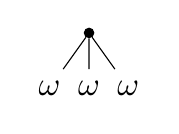
\begin{tikzpicture}
    \node[int] (i) at (0,.5) {};
    \node (v1) at (-.5,-.2) {$\omega$};
    \node (v2) at (0,-.2) {$\omega$};
    \node (v3) at (.5,-.2) {$\omega$};
  \draw (i) edge (v1) edge (v2) edge (v3);
  \end{tikzpicture}
}
\newcommand{\tripods}{
\tripod 
\cdots 
\tripod
}

%%%%%%%%%%%%%%%%%%%%%%%%%%%%%%%%%%%
%%%%%%%%%%%%%%%%%%%%%%%%%%%%%%%%%%%%




\newcommand{\sam}[1]{{ \sf $\diamondsuit\diamondsuit\diamondsuit$ {\textcolor{red}{Sam: [#1]}}}}

\newcommand{\thomas}[1]{{ \sf $\diamondsuit\diamondsuit\diamondsuit$ {\textcolor{magenta}{Thomas: [#1]}}}}

\newcommand{\newtext}[1]{{ {\textcolor{blue}{#1}}}}


\newcommand{\hannah}[1]{{\color{teal} ($\spadesuit$ Hannah: #1)}}
\newcommand{\samc}[1]{{\color{red} ($\spadesuit$ Sam C: #1)}}
\newcommand{\samp}[1]{{\color{violet} ($\spadesuit$ Sam P: #1)}}


\usepackage{color, colortbl}
\usepackage{array, adjustbox}

\definecolor{Gray}{gray}{0.9}

\newcolumntype{g}{>{\columncolor{Gray}}c}
\newcolumntype{M}{V{6cm}} %M is for Maximal column
\newcolumntype{N}{V{12cm}} %M is for Maximal column

\author{Marco Belli}
\author{Thomas Willwacher}

% \thanks{
% thanks note and support.....
% }





\title{Getzler-Kapranov Graph Complex cohomology computations in low excesses}



\begin{document}

\begin{abstract}
    We carry out computations in the Getzler-Kapranov graph complex in weight $13$ following the approach of \cite{CLPW2} by classifying graphs using the excess $e(g,n)=3(g-1)+2n-22$ as complexity function. The classification is automated in Python using SageMath.
\end{abstract}

\maketitle

%\setcounter{tocdepth}{1}
%\tableofcontents








\section{Introduction}

The authors of \cite{CLPW2} study the weight graded pieces of $H^*_c(\M_{g,n})$ using graph complexes. The associated graded of the weight filtration is identified with the cohomology of the modular cooperad whose $(g,n)$ part is $H^*(\Mb_{g,n})$, it is known as the Getzler-Kapranov graph complex:
\begin{equation}
    H^*(\GK_{g,n}^k) \cong  \gr^W_k H^*_c(\M_{g,n}) := W_k H^*_c(\M_{g,n})/W_{k-1}H^*_c(\M_{g,n})
\end{equation}

They obtain two following results in weight 13.
\begin{prop}\label{prop:wt 13 vanishing}
    If $3g + 2n \leq 25$ then $\gr_{13}^W H^*_c(\M_{g,n}) = 0$.
\end{prop}

\begin{thm} \label{thm:lowexc13}
    Suppose $3g + 2n \in \{26, 27\}$. Then $\gr_{13}^W H^*_c(\M_{g,n})$ is nonzero only in degree $$k(g,n) = 3g + n - 2 - \delta_{0,n},$$ and there is an $\ss_n$-equivariant isomorphism $\gr_{13}^W H^{k(g,n)}_c(\cM_{g,n}) \cong Z_{g,n} \otimes \lstw$, where
\begin{align*}
    Z_{1,12} & \cong V_{21^{10}} & Z_{2,10} & \cong V_{1^{10}} & Z_{3,9} & \cong V_{1^{9}} \\
    Z_{4,7} & \cong V_{1^{7}} & Z_{5,6} & \cong V_{1^{6}} \oplus V_{21^4}^{\oplus 2} & Z_{6,4} & \cong V_{1^{4}} \\ Z_{7,3} & \cong V_{1^{3}} \oplus V_{21}^{\oplus 2}& Z_{8,1} & \cong \Q & Z_{9,0} & \cong \Q 
\end{align*}
\end{thm}

With our computations we extend to the following case.
\begin{thm} \label{thm:excess28}
    Suppose $3g + 2n =28$. Then $\gr_{13}^W H^*_c(\M_{g,n})$ vanishes outside the degrees $$k_1(g,n) = 3g + n - 2 \hspace{.5cm}\text{and}\hspace{.5cm} k_2(g,n) = 3g + n - 3$$ and there are $\ss_n$-equivariant isomorphisms $$ \gr_{13}^W H^{k_1(g,n)}_c(\cM_{g,n}) \cong Z_{g,n} \otimes \lstw  \hspace{1cm} \gr_{13}^W H^{k_2(g,n)}_c(\cM_{g,n}) \cong W_{g,n} \otimes \lstw , $$ where
\begin{align*}
    Z_{2,11} &\cong V_{21^{9}}\oplus V_{221^7} \oplus V_{31^8}^{\oplus 2} & Z_{4,8} &\cong V_{21^6}\oplus V_{221^4}\oplus V_{31^5}^{\oplus 3} & Z_{6,5} &\cong V_{21^3}\oplus V_{221}\oplus V_{31^2}^{\oplus 3}
\end{align*}
\begin{align*}
    Z_{8,2}&=0 &  W_{2,11}&=V_{1^{11}}^{\oplus 2} & W_{4,8}&=V_{1^8}^{\oplus 2} & W_{6,5}&=V_{1^5}^{\oplus 2} & W_{8,2}&=V_{1^2}
\end{align*}
\end{thm}




\section{Graph Complexes in weight 13}

In this sections, we recall the definition of the Getzler-Kapranov graph complex and its simplified version obtained as a quasi-isomorphic quotient in \cite{CLPW2}. Then we model combinatorially it's weight 13 graded piece using the graphical depictions of generators of the cohomology groups $H^{12,1}(\MM_{1,n})$, $H^{11,0}(\MM_{1,n})$, $H^{1,1}(\MM_{g,n})$.

\subsection{The simplified Getzler-Kapranov graph complex in weight 13}
In the following we will consider stable graphs $\Gamma\in\Gamma((g,n))$ equipped with a decoration $(\gamma_v)_{v\in V(\Gamma)}$ of their vertices by cohomology classes $\gamma_v \in H^{*}(\MM_{g_v,n_v})$ which behaves tensorially in $v$, and with an alternating ordering of the internal edges $(o_e)_{e\in E(\Gamma)}$; we will refer to such graphs $(\Gamma,\gamma\otimes o)$ shortly as \emph{decorated graphs}. Isomorphisms $\phi:\Gamma\xrightarrow{\sim}\Gamma'$ of stable graphs act on the decorated graphs with underlying graph $\Gamma$ by permutation:
\[ \phi_* (\Gamma,(\gamma_v)_{v}\otimes (o_e)_{e}) = (\Gamma',(\gamma_v)_{\phi(v)}\otimes (o_e)_{\phi(e)}). \]

The Getzler-Kapranov graph complex has a presentation by the space of coinvariants of decorated graphs under isomorphisms:
\begin{multline}\label{equ:GKdef}
    \GK_{g,n} = 
    \bigg( \bigoplus_{\Gamma\in\Gamma((g,n))} \bigotimes_{v\in V(\Gamma)}H^{*}(\MM_{g_v,n_v})\otimes \Q[-1]^{\otimes |E(\Gamma)|} \bigg) \Big/ \sim \\
    = \bigoplus_{[\Gamma]\in[\Gamma((g,n))]} \bigg(
    \bigotimes_{v\in V(\Gamma)}H^{*}(\MM_{g_v,n_v})\otimes \Q[-1]^{\otimes |E(\Gamma)|} \bigg) \Big/ \text{Aut}_{\Gamma},
\end{multline}
where the $\Gamma((g,n))$ are stable graphs and $[\Gamma((g,n))]$ their isomorphism classes, of which there are only finitely for every pair $(g,n)$. Automorphisms of stable graphs are understood to fix the $n$ labeled hairs and to act by the sign of their induced permutation on the internal edges $E(\Gamma)$.

The \emph{weight} of a decorated graph $(\Gamma,\gamma\otimes o)$ with all $\gamma_v$ of pure cohomological degree $k_v$ is $\kappa=\sum_v k_v$. For each $\kappa\in\NN$, the homogeneous slice of weight $\kappa$ of $\GK_{g,n}$ is then given by 
\begin{equation}\label{equ:GKweight}
    \GK^{\kappa}_{g,n} 
    = \bigoplus_{[\Gamma]\in[\Gamma((g,n))]} \bigoplus_{\substack{\lambda\,\text{partition} \\ \text{of}\,\kappa}} \bigg( \bigoplus_{\substack{k:V(\Gamma)\rightarrow \NN \\ k\,\text{respects}\,\lambda}}
    \bigotimes_{v\in V(\Gamma)}H^{k_v}(\MM_{g_v,n_v})\otimes \Q[-1]^{\otimes |E(\Gamma)|} \bigg) \Big/ \text{Aut}_{\Gamma},
\end{equation}

The grading of the complex $\GK_{g,n}$ is given by the weight plus the number of internal edges of the stable graphs. For the definition of the differential we refer to \cite{CLPW2}; in \ref{subsec:differential} we will describe its action on the graphical depictions of the generators.

Since $H^{k}(\MM_{g,n})=0$ for odd $k<11$ \cite{BergstromFaberPayne}, the only weight labelings $k:V(\Gamma)\rightarrow\NN$ with $13=\sum_v k_v$ giving rise to non trivial decorated graphs are the ones with zero weight on every vertex except either $(A)$ $k_{\bar{v}}=13$ or $(B)$ $k_{\bar{v}}=11$, $k_{\tilde{v}}=2$ for exactly one special vertex $\bar{v}$ and in case $(B)$ a second vertex $\tilde{v}$. We will denote by $N_{\bar{v}}$ and $N_{\tilde{v}}$ the hairs and half-edges at $\bar{v}$ and $\tilde{v}$. We can reduce further the coinvariants by summing over all possible choices of $\bar{v}$ in case $(A)$ and $\bar{v},\tilde{v}$ in case $(B)$, and requiring that automorphisms fix these vertices:

\begin{multline}\label{equ:GK13}
    \GK^{13}_{g,n}
    = \bigoplus_{\substack{ [\Gamma]\in[\Gamma((g,n))] \\ \bar{v}\in V(\Gamma)}}
    \left( H^{13}(\MM_{g_{\bar{v}},n_{\bar{v}}}) \otimes \Q[-1]^{\otimes |E(\Gamma)|} \right)/\text{Aut}_{\Gamma,\bar{v}} \\
    \oplus \bigoplus_{\substack{ [\Gamma]\in[\Gamma((g,n))] \\ \bar{v}\neq\tilde{v}\in V(\Gamma)}}
    \left( H^{11}(\MM_{g_{\bar{v}},n_{\bar{v}}}) \otimes H^{2}(\MM_{g_{\tilde{v}},n_{\tilde{v}}}) \otimes \Q[-1]^{\otimes |E(\Gamma)|} \right)/\text{Aut}_{\Gamma,\bar{v},\tilde{v}} .
\end{multline}
% \[  \GK^{13}_{g,n} 
%     = \bigoplus_{\substack{ [\Gamma]\in[\Gamma((g,n))] \\ \bar{v}\in V(\Gamma) \\ \text{no odd symmetries} \\ \text{fixing}\,\bar{v} }}
%     H^{13}(\MM_{g_{\bar{v}},n_{\bar{v}}}) \;\oplus
%     \bigoplus_{\substack{ [\Gamma]\in[\Gamma((g,n))] \\ \bar{v}\neq\tilde{v}\in V(\Gamma) \\ \text{no odd symmetries} \\ \text{fixing}\,\bar{v},\tilde{v} }}
%     H^{11}(\MM_{g_{\bar{v}},n_{\bar{v}}}) \otimes H^{2}(\MM_{g_{\tilde{v}},n_{\tilde{v}}}) \]


As the cohomology groups come equipped with a $\Q$-Hodge decomposition \ref{thm:GroupsHodgeDeco}, we obtain accordingly a decomposition $\GK_{g,n}^{13}\otimes\CC = \GK_{g,n}^{12,1} \oplus \GK_{g,n}^{1,12}$, where $\GK_{g,n}^{12,1}$ is obtained as in \ref{equ:GK13} by replacing $H^{13}, H^{11}$ and $H^{2}$ by $H^{12,1}, H^{11,0}$ and $H^{1,1}$ respectively. After quotienting by an appropriate subspace closed under the differential, we obtain a quasi-isomorphic complex $\GK_{g,n}^{13}\twoheadrightarrow \bGK_{g,n}^{13}$ generated by a much smaller set of decorated graphs \cite[Section 2.2]{CLPW2}. This quasi-isomorphism preserves the above $\Q$-Hodge decomposition: $\bGK_{g,n}^{13}\otimes\CC = \bGK_{g,n}^{12,1} \oplus \bGK_{g,n}^{1,12}$. From now on we will focus on the $\bGK_{g,n}^{12,1}$ part, which is generated by the subset of decorated graphs satisfying the following properties:

\begin{enumerate}
    \item[1)] Weight zero vertices have genus zero, valence at least $3$ and don't have loops.
    \item[2)] In both cases $(A)$ and $(B)$ the special vertex $\bar{v}$ has $g_{\bar{v}}=1$.
    \item[2b)] In case $(B)$ the special vertex $\tilde{v}$ has either $g_{\tilde{v}}=0$, or $g_{\tilde{v}}=1$ and $n_{\tilde{v}}=1$.
\end{enumerate}

Using the presentation of the cohomology groups described in \ref{sec:appendix}, we consider the subspace of  $\GK_{g,n}^{12,1}$  spanned by generators with propreties $1),2),2b)$ and we exchange the order of the cohomology relations and the coinvariants relations to obtain 
\begin{multline}\label{equ:GK12,1}
    \bGK_{g,n}^{12,1}  \twoheadleftarrow  \bigoplus_{\substack{[\Gamma],\bar{v},\,B\subseteq A\subseteq N_{\bar{v}} \\ |B|=10, |A^c|\geq 3}} \left( \left<Z_{B\subseteq A}\right> \otimes \Q[-1]^{\otimes |E(\Gamma)|} \right)/\text{Aut}_{\Gamma,\bar{v}}^{B,A} \\
    \oplus \bigoplus_{\substack{[\Gamma],\bar{v},\,E\subseteq N_{\bar{v}} \\ |E|=12}} \bigg( \bigoplus_{\substack{B\subseteq A\subseteq N_{\bar{v}} \\  B\sqcup A^c=E}} \left( \left<Z_{B\subseteq A}\right> \otimes \Q[-1]^{\otimes |E(\Gamma)|} \right)/\text{Aut}_{\Gamma,\bar{v}}^{B,A} \bigg) \Big/ \{\substack{\text{weight 13}\\\text{relations}}\} \\
    \oplus \bigoplus_{[\Gamma],\bar{v},\tilde{v}} \bigg( \bigoplus_{\substack{B\subseteq N_{\tilde{v}},|B|=11\\ A\sqcup A'=N_{\tilde{v}},|A|,|A'|\geq 2}} \left( \left<\omega_B\otimes\delta\{\substack{A \\ A'}\}\right> \otimes \Q[-1]^{\otimes |E(\Gamma)|}\right) / \text{Aut}_{\Gamma,\bar{v},\tilde{v}}^{B,\{A,A'\} } \bigg) \Big/ \{\substack{\text{weight 11 and 2}\\\text{relations}}\} \\
    \oplus \bigoplus_{[\Gamma],\bar{v},\tilde{v}} \bigg( \bigoplus_{\substack{B\subseteq N_{\tilde{v}}\\ |B|=11}} \left( \left<\omega_B\otimes \delta_{irr}\right> \otimes \Q[-1]^{\otimes |E(\Gamma)|}\right) / \text{Aut}_{\Gamma,\bar{v},\tilde{v}}^B \bigg) \Big/ \{\substack{\text{weight 11}\\\text{relations}}\} ,
\end{multline}
where, for example in the third term, Aut$_{\Gamma,\bar{v},\tilde{v}}^{B,\{A,A'\}}$ is the group of automorphisms leaving the set $B$ and the partition $A\sqcup A'$ invariant.
These are precisely the symmetries of the decorated graphs $(\Gamma,Z_{B\subseteq A}\otimes o)$, $(\Gamma,\omega_B\otimes\delta\{\substack{A \\ A'}\}\otimes o)$ and $(\Gamma,\omega_B\otimes \delta_{irr}\otimes o)$ respectively, which act by the sign of the permutation of the half-edges of $\bar{v}$ in $B$ multiplied by the sign of the permutation on the internal edges $E(\Gamma)$. In each case, the coinvariants relations restrict to killing the decorated graphs with odd symmetry. In the following we will consider the familiy of generators indexed by all the direct sums in \ref{equ:GK12,1} whose automorphism group does not have odd symmetries. In particular we can impose the further restriction on the generators:
\begin{enumerate}
    \item[1.2)] There are no multiple edges, except possibly for edges incident at $\bar{v}$ or $\tilde{v}$.
\end{enumerate}

The relations introduced by the quotient manifest as follows between the generators:\\
\begin{minipage}[t]{0.44\textwidth}
Case $(A)$:
\begin{enumerate}
    \item[3a)] Graphs with a loop $(s,t)$ at $\bar{v}$ and decorated by a $Z_{B\subseteq A}$ with $|A^c|\geq 3$, $s,t\in A^c$ are set to zero.
\end{enumerate}
\end{minipage}
\begin{minipage}[t]{0.56\textwidth}
Case $(B)$:
\begin{enumerate}
    \item[3b)] Graphs with $g_{\tilde{v}}=0$ and a loop at $\tilde{v}$ decorated by a class in the image of the pullback $H^2(\MM_{1,n_{\tilde{v}}-2})\xrightarrow{\xi_{*}} H^2(\MM_{0,n_{\tilde{v}}})$ are set to zero. 
\end{enumerate}
\end{minipage}%
\begin{enumerate}
    \item[4)] Case $(A)$ graphs with a loop $(s,t)$ at $\bar{v}$ and decorated by a $Z_{B\subseteq A}$ with $A^c=\{s,t\}$ are identified with $\frac{1}{12}$ times the case $(B)$ graph obtained by adding a genus $1$ vertex $\tilde{v}$, connecting it only to $\bar{v}$ through an edge $(p',p)$, redecorating $\bar{v}$ with the weight $11$ class $\omega_{B\sqcup p}$ and decorating $\tilde{v}$ with the weight $2$ class $\delta_{irr}$.
\end{enumerate}

We represent these relations using the graphical depictions of cohomology classes in \ref{sec:appendix}. When talking about the depiction, the genus one vertex and the two ends of the crossed edge will be referenced by the keys $\bar{v}$ and $\tilde{v}$ in case $(A)$ and  $\bar{v}$,$\tilde{v}_1$ and $\tilde{v}_2$ in case $(B)$.

\[
    \text{3b): }
    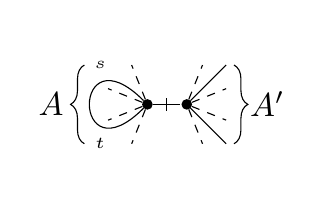
\begin{tikzpicture}
        \node[int] (v) at (0,0) {};
        \node[int] (w) at (0.5,0) {};
        \node (s) at (-.6,.5)  {\tiny$s$};
        \node (t) at (-.6,-.5)  {\tiny$t$};
        \draw (v) to [out=135,in=225,distance=1.3cm] (v) edge[dashed] +(-.5,.2) edge[dashed] +(-.2,.5) edge[dashed] +(-.5,-.2) edge[dashed] +(-.2,-.5) edge[crossed] (w)
        (w) edge +(.5,-.5) edge +(.5,.5) edge[dashed] +(.5,.2) edge[dashed] +(.5,-.2) edge[dashed] +(.2,.5) edge[dashed] +(.2,-.5);
        \draw [decorate,decoration={brace,amplitude=5pt,mirror}]
        (-.8,.5) -- (-.8,-.5) node[midway,xshift=-1em]{$A$};
        \draw [decorate,decoration={brace,amplitude=5pt}]
        (1.1,.5) -- (1.1,-.5) node[midway,xshift=1em]{$A'$};
    \end{tikzpicture}
    = 0
    \hspace{1cm}
    \sum_{\substack{A\sqcup A'= N_{\tilde{v}}\\ |A|,|A'|\geq 2 \\ s\in A, t\in A'}}
    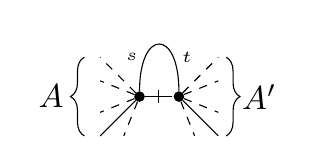
\begin{tikzpicture}
        \node[int] (v) at (0,0) {};
        \node[int] (w) at (0.5,0) {};
        \node (s) at (-.1,.5)  {\tiny$s$};
        \node (t) at (.6,.5)  {\tiny$t$};
        \draw (v) edge +(-.5,-.5) edge[dashed] +(-.5,.5) edge[dashed] +(-.5,.2) edge[dashed] +(-.5,-.2) edge[dashed] +(-.2,-.5) edge[crossed] (w) edge[bend left=90,distance=.8cm] (w)
        (w) edge +(.5,-.5) edge[dashed] +(.5,.5) edge[dashed] +(.5,.2) edge[dashed] +(.5,-.2) edge[dashed] +(.2,-.5);
        \draw [decorate,decoration={brace,amplitude=5pt,mirror}]
        (-.7,.5) -- (-.7,-.5) node[midway,xshift=-1em]{$A$};
        \draw [decorate,decoration={brace,amplitude=5pt}]
        (1.1,.5) -- (1.1,-.5) node[midway,xshift=1em]{$A'$};
    \end{tikzpicture}
    =0
\]

\[
    \text{3a) and 4):  }
    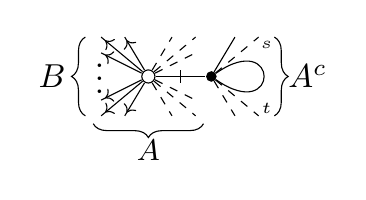
\begin{tikzpicture}
        \node[ext] (v) at (0,0) {};
        \node at (-.62, .1) {$\scriptscriptstyle \vdots$};
        \node[int] (w) at (.8, 0) {};
        \node (s) at (1.5,.4) {\tiny$s$};
        \node (t) at (1.5,-.4) {\tiny$t$};
        \draw (v) edge[->-] +(-.6,-.5) edge[->-] +(-.6,-.3) edge[->-] +(-.3,-.5)
        edge[->-] +(-.6,.5) edge[->-] +(-.6,.3) edge[->-] +(-.3,.5) 
        edge[dashed] +(.6,.5) edge[dashed] +(.6,+.3)  edge[dashed] +(.3,+.5)
        edge[dashed] +(.6,-.5) edge[dashed] +(.6,-.3) edge[dashed] +(.3,-.5) edge[crossed] (w);
        \draw (w)  to [out=35,in=-35,distance=1cm] (w) edge[dashed] +(.6,+.5)  edge +(.3,+.5)
        edge[dashed] +(.6,-.5) edge[dashed] +(.3,-.5);
        \draw [decorate,decoration={brace,amplitude=5pt,mirror}]
        (-.8,.5) -- (-.8,-.5) node[midway,xshift=-1em]{$B$};
        \draw [decorate,decoration={brace,amplitude=5pt}]
        (1.6,.5) -- (1.6,-.5) node[midway,xshift=1em]{$A^c$};
        \draw [decorate,decoration={brace,mirror,amplitude=5pt}]
        (-.7,-.6) -- (.7,-.6) node[midway,yshift=-0.8em]{\small $A$};
    \end{tikzpicture}
    =0
    \hspace{0.8cm}
    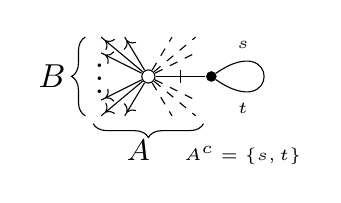
\begin{tikzpicture}
        \node[ext] (v) at (0,0) {};
        \node at (-.62, .1) {$\scriptscriptstyle \vdots$};
        \node[int] (w) at (.8, 0) {};
        \node (s) at (1.2,.4) {\tiny$s$};
        \node (t) at (1.2,-.4) {\tiny$t$};
        \draw (v) edge[->-] +(-.6,-.5) edge[->-] +(-.6,-.3) edge[->-] +(-.3,-.5)
        edge[->-] +(-.6,.5) edge[->-] +(-.6,.3) edge[->-] +(-.3,.5) 
        edge[dashed] +(.6,.5) edge[dashed] +(.6,+.3)  edge[dashed] +(.3,+.5)
        edge[dashed] +(.6,-.5) edge[dashed] +(.6,-.3) edge[dashed] +(.3,-.5) edge[crossed] (w);
        \draw (w)  to [out=35,in=-35,distance=1cm] (w);
        \draw [decorate,decoration={brace,amplitude=5pt,mirror}]
        (-.8,.5) -- (-.8,-.5) node[midway,xshift=-1em]{$B$};
        \draw [decorate,decoration={brace,mirror,amplitude=5pt}]
        (-.7,-.6) -- (.7,-.6) node[midway,xshift=-.3em,yshift=-0.8em]{\small $A$};
        \node at (1.2,-1) {\tiny $A^c=\{s,t\}$};
    \end{tikzpicture}
    =
    \frac{1}{12}
    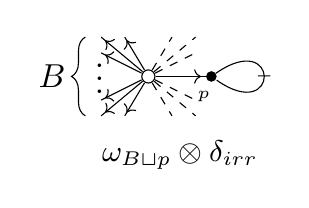
\begin{tikzpicture}
        \node[ext] (v) at (0,0) {};
        \node at (-.62, .1) {$\scriptscriptstyle \vdots$};
        \node[int] (w) at (.8, 0) {};
        \node at (.7,-.25) {\tiny$p$};
        \node at (.4,-1) {\small$\omega_{B\sqcup p}\otimes\delta_{irr}$};
        \draw (v) edge[->-] +(-.6,-.5) edge[->-] +(-.6,-.3) edge[->-] +(-.3,-.5)
        edge[->-] +(-.6,.5) edge[->-] +(-.6,.3) edge[->-] +(-.3,.5) 
        edge[dashed] +(.6,.5) edge[dashed] +(.6,+.3)  edge[dashed] +(.3,+.5)
        edge[dashed] +(.6,-.5) edge[dashed] +(.6,-.3) edge[dashed] +(.3,-.5) edge[->-] (w);
        \draw (w) edge[crossed, out=35,in=-35,distance=1cm] (w);
        \draw [decorate,decoration={brace,amplitude=5pt,mirror}]
        (-.8,.5) -- (-.8,-.5) node[midway,xshift=-1em]{$B$};
    \end{tikzpicture}
\]

With condition $1)$ and relations $3a),3b), 4)$ we can consider only the generators whose graphical depiction has no loops except possibly at $\bar{v}$, but including the special case of exactly one loop at $\tilde{v}$ for the case $(B)$ with $\omega_B\otimes \delta_{irr}$. In addition, we can ignore case $(A)$ generators with $|A^c|=2$ and a multiple edge parallel to the crossed edge with an endpoint in the set $B$ using coinvariants and the weight $13$ relation:
\[
    2 \cdot
    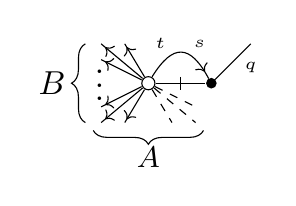
\begin{tikzpicture}
        \node[ext] (v) at (0,0) {};
        \node at (-.62, .1) {$\scriptscriptstyle \vdots$};
        \node[int] (w) at (.8, 0) {};
        \node (q) at (1.3,.2) {\tiny$q$};
        \node (s) at (.65,.5) {\tiny$s$};
        \node (t) at (.15,.5) {\tiny$t$};
        \draw (v) edge[->-] +(-.6,-.5) edge[->-] +(-.6,-.3) edge[->-] +(-.3,-.5)
        edge[->-] +(-.6,.5) edge[->-] +(-.6,.3) edge[->-] +(-.3,.5) 
        edge[dashed] +(.6,-.5) edge[dashed] +(.6,-.3) edge[dashed] +(.3,-.5) edge[crossed] (w) edge[->-, bend left=60,distance=.5cm] (w);
        \draw (w) edge +(.5,+.5);
        \draw [decorate,decoration={brace,amplitude=5pt,mirror}]
        (-.8,.5) -- (-.8,-.5) node[midway,xshift=-1em]{$B$};
        \draw [decorate,decoration={brace,mirror,amplitude=5pt}]
        (-.7,-.6) -- (.7,-.6) node[midway,yshift=-0.8em]{\small $A$};
    \end{tikzpicture}
    =
    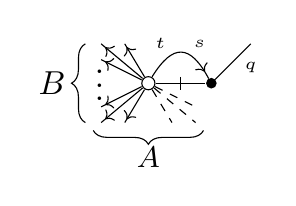
\begin{tikzpicture}
        \node[ext] (v) at (0,0) {};
        \node at (-.62, .1) {$\scriptscriptstyle \vdots$};
        \node[int] (w) at (.8, 0) {};
        \node (q) at (1.3,.2) {\tiny$q$};
        \node (s) at (.65,.5) {\tiny$s$};
        \node (t) at (.15,.5) {\tiny$t$};
        \draw (v) edge[->-] +(-.6,-.5) edge[->-] +(-.6,-.3) edge[->-] +(-.3,-.5)
        edge[->-] +(-.6,.5) edge[->-] +(-.6,.3) edge[->-] +(-.3,.5) 
        edge[dashed] +(.6,-.5) edge[dashed] +(.6,-.3) edge[dashed] +(.3,-.5) edge[crossed] (w) edge[->-, bend left=60,distance=.5cm] (w);
        \draw (w) edge +(.5,+.5);
        \draw [decorate,decoration={brace,amplitude=5pt,mirror}]
        (-.8,.5) -- (-.8,-.5) node[midway,xshift=-1em]{$B$};
        \draw [decorate,decoration={brace,mirror,amplitude=5pt}]
        (-.7,-.6) -- (.7,-.6) node[midway,yshift=-0.8em]{\small $A$};
    \end{tikzpicture}
    +
    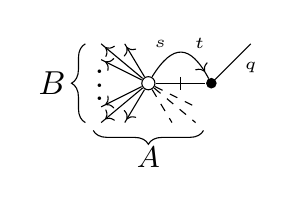
\begin{tikzpicture}
        \node[ext] (v) at (0,0) {};
        \node at (-.62, .1) {$\scriptscriptstyle \vdots$};
        \node[int] (w) at (.8, 0) {};
        \node (q) at (1.3,.2) {\tiny$q$};
        \node (s) at (.65,.5) {\tiny$t$};
        \node (t) at (.15,.5) {\tiny$s$};
        \draw (v) edge[->-] +(-.6,-.5) edge[->-] +(-.6,-.3) edge[->-] +(-.3,-.5)
        edge[->-] +(-.6,.5) edge[->-] +(-.6,.3) edge[->-] +(-.3,.5) 
        edge[dashed] +(.6,-.5) edge[dashed] +(.6,-.3) edge[dashed] +(.3,-.5) edge[crossed] (w) edge[->-, bend left=60,distance=.5cm] (w);
        \draw (w) edge +(.5,+.5);
        \draw [decorate,decoration={brace,amplitude=5pt,mirror}]
        (-.8,.5) -- (-.8,-.5) node[midway,xshift=-1em]{$B$};
        \draw [decorate,decoration={brace,mirror,amplitude=5pt}]
        (-.7,-.6) -- (.7,-.6) node[midway,yshift=-0.8em]{\small $A$};
    \end{tikzpicture}
    =
    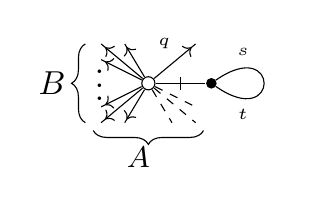
\begin{tikzpicture}
        \node[ext] (v) at (0,0) {};
        \node at (-.62, .1) {$\scriptscriptstyle \vdots$};
        \node[int] (w) at (.8, 0) {};
        \node (q) at (.2,.5) {\tiny$q$};
        \node (s) at (1.2,.4) {\tiny$s$};
        \node (t) at (1.2,-.4) {\tiny$t$};
        \draw (v) edge[->-] +(-.6,-.5) edge[->-] +(-.6,-.3) edge[->-] +(-.3,-.5)
        edge[->-] +(-.6,.5) edge[->-] +(-.6,.3) edge[->-] +(-.3,.5) 
        edge[->-] +(.6,.5)
        edge[dashed] +(.6,-.5) edge[dashed] +(.6,-.3) edge[dashed] +(.3,-.5) edge[crossed] (w);
        \draw (w)  to [out=35,in=-35,distance=1cm] (w);
        \draw [decorate,decoration={brace,amplitude=5pt,mirror}]
        (-.8,.5) -- (-.8,-.5) node[midway,xshift=-1em]{$B$};
        \draw [decorate,decoration={brace,mirror,amplitude=5pt}]
        (-.7,-.6) -- (.7,-.6) node[midway,xshift=-.3em,yshift=-0.8em]{\small $A$};
    \end{tikzpicture}.
\]


Considering now the graphical depictions, we obtain four families of $(g,n)$-stable graphs with features, which we call $A_3,A_2,B_1$ and $B_{irr}$; denote graphs with features in these families as $G_{\bar{v},B\subseteq A}^{\tilde{v}}$, $G_{\bar{v},B}^{\tilde{v}_1,\tilde{v}_2}$, $G_{\bar{v},B}^{\tilde{v},irr}$. The variables range in each case over the following objects:
\begin{enumerate}
    \item[all:\, ] Any $(g,n)$-stable graph $G$ with exactly one genus $1$ vertex $\bar{v}$ and every other vertex having genus $0$.
    \item[$A_3,A_2$: ] Any choice of a crossed internal edge ($\bar{v},\tilde{v}$) adjacent to $\bar{v}$. In this case, with $N_{\bar{v}}$ we will always mean the hairs and half-edges adjacent to $\bar{v}$ or to $\tilde{v}$ excluding the two crossed half-edges, and we fix a canonical ordering of the set $N_{\bar{v}}$. In addition, there's any choice of subsets $B\subseteq A\subseteq N_{\bar{v}}$ with $|B|=10$ and either $|A^c|\geq 3$ or $|A^c|=2$, called $A_3$ and $A_2$ cases respectively. $G$ is required to be simple, except possibly with loops at $\bar{v}$ or multiple edges parallel to the crossed edge.
    \item[$B_1,B_{irr}$: ] Any choice of subset $B\subseteq N_{\bar{v}}$ with $|B|=11$.  We fix a canonical ordering on $N_{\bar{v}}$.
    \item[$B_1$:] Any choice of a crossed internal edge $\tilde{v}=(\tilde{v}_1,\tilde{v}_2)$ not adjacent to $\bar{v}$, in this case we denote by $N_{\tilde{v}}$ the hairs and half-edges adjacent to $\tilde{v}_1$ or $\tilde{v}_2$ excluding the two crossed half-edges. $G$ is required to be simple, except possibly with loops at $\bar{v}$ or multiple edges parallel to the crossed edge.
    \item[$B_{irr}$:] $G$ is required to be simple, except possibly with loops at $\bar{v}$, and with exactly one vertex $\tilde{v}\neq\bar{v}$ with unique neighbour $\bar{v}$ and one loop, which we call the crossed edge.
    \item[all:\,] A choice of alternating order of the internal edges of $G$ which are not crossed.
    \item[all:\,] The resulting graph with features must have no odd symmetries. Here a symmetry is a graph automorphism that preserves all the choices made above.
\end{enumerate}

The only relations amongst these four families of generators are the relations of the cohomology classes $Z_{B\subseteq A}$ in case $A_2$ and $\omega_B$ in case $B_1,B_{irr}$ and the remaining quotient relation 3b) in case $B_1$, which can be seen as just an extension of the weight $2$ relations. Using these four families of generators, we obtain
\begin{multline}
    \; \bGK^{12,1}_{g,n} = \;\;
    \bigoplus_{\left[\substack{G,\bar{v},\tilde{v} \\ B,A,|A^c|\geq 3} \right]} \left< G_{\bar{v},B\subseteq A}^{\tilde{v}} \right>
    \oplus \bigg( \bigoplus_{\left[\substack{G,\bar{v},\tilde{v} \\ B,A,|A^c|=2 }\right]} \left< G_{\bar{v},B\subseteq A}^{\tilde{v}} \right> \bigg) \bigg/ \{\substack{\text{weight 13}\\ \text{relations}}\} \\
    \oplus \bigg( \bigoplus_{\left[\substack{G,\bar{v},\tilde{v} \\ B, A}\right]} \left<G_{\bar{v},B}^{\tilde{v},\{A,A'\}} \right> \bigg) \bigg/ \{\substack{\text{weight 11, 2, and}\\ \text{$3b)$ relations}}\}
    \oplus \bigg( \bigoplus_{\left[G,\bar{v},\tilde{v},B\right]} \left< G_{\bar{v},B}^{\tilde{v},irr} \right> \bigg) \bigg/ \{\substack{\text{weight 11}\\ \text{relations}}\},
\end{multline}
where the square brackets indicate that we range over all the admissible choices listed above, up to isomorphisms of graphs with these features.


\subsection{Blown-up representation of the generators}
In order to determine $\bGK_{g,n}^{12,1}$, we need to classify the four families of graphs with features above up to isomorphism. To this end, we look at their connected components after deleting the special vertex but keeping it's half-edges and hairs; this is called the blown-up representation. We keep track of the features at the special vertex by labeling the hairs of the blown-up components either $\epsilon$ or $\omega$; in each case there are precisely eleven $\omega$ labels. In the pictures below, one has to imagine  the rest of the ambient graph to exist unchanged, potentially grouping the $\epsilon$ and $\omega$ hairs into connected components.

\[
    G_{\bar{v},B}^{\tilde{v},\{A,A'\}},G_{\bar{v},B}^{\tilde{v},irr} 
     \mapsto G_{\bar{v},B}^{\tilde{v},\{A,A'\}}\setminus \bar{v}, G_{\bar{v},B}^{\tilde{v},irr}  \setminus \bar{v} \hspace{3cm}
     G_{\bar{v},B\subseteq A}^{\tilde{v}} \hspace{.5cm} \mapsto \hspace{.4cm} G_{\bar{v},B\subseteq A}^{\tilde{v}}\setminus \bar{v} \hspace{1cm}
\]
\[
    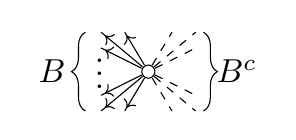
\begin{tikzpicture}
        \node[ext] (v) at (0,0) {};
        \node at (-.62, .1) {$\scriptscriptstyle \vdots$};
        \draw (v) edge[->-] +(-.6,-.5) edge[->-] +(-.6,-.3) edge[->-] +(-.3,-.5)
        edge[->-] +(-.6,.5) edge[->-] +(-.6,.3) edge[->-] +(-.3,.5) 
        edge[dashed] +(.6,.5) edge[dashed] +(.6,+.3)  edge[dashed] +(.3,+.5)
        edge[dashed] +(.6,-.5) edge[dashed] +(.6,-.3) edge[dashed] +(.3,-.5) ;
        \draw [decorate,decoration={brace,amplitude=5pt,mirror}]
      (-.8,.5) -- (-.8,-.5) node[midway,xshift=-1em]{$B$};
        \draw [decorate,decoration={brace,amplitude=5pt}]
        (.7,.5) -- (.7,-.5) node[midway,xshift=1em]{$B^c$};
    \end{tikzpicture}
    \mapsto
    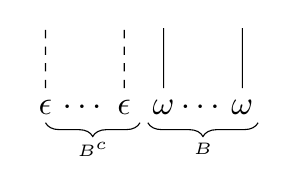
\begin{tikzpicture}
        \node (e1) at (-1.5,-.5) {$\epsilon$};
        \node at (-1,-.5) {$\dots$};
        \node (e2) at (-.5,-.5) {$\epsilon$};
        \node (w1) at (0,-.5) {$\omega$};
        \node at (0.5,-.5) {$\dots$};
        \node (w2) at (1,-.5) {$\omega$};
        \draw (e1) edge[dashed] +(0,1) (e2) edge[dashed] +(0,1);
        \draw (w1) edge +(0,1) (w2) edge +(0,1);
        \draw [decorate,decoration={brace,mirror,amplitude=5pt}]
        (-1.5,-.7) -- (-.3,-.7) node[midway,yshift=-0.8em]{\tiny $B^c$};
        \draw [decorate,decoration={brace,mirror,amplitude=5pt}]
        (-.2,-.7) -- (1.2,-.7) node[midway,yshift=-0.8em]{\tiny $B$};
    \end{tikzpicture}
    \hspace{0.6cm}
    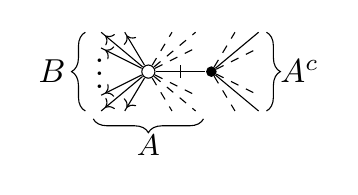
\begin{tikzpicture}
        \node[ext] (v) at (0,0) {};
        \node at (-.62, .1) {$\scriptscriptstyle \vdots$};
        \node[int] (w) at (.8, 0) {};
        \draw (v) edge[->-] +(-.6,-.5) edge[->-] +(-.6,-.3) edge[->-] +(-.3,-.5)
        edge[->-] +(-.6,.5) edge[->-] +(-.6,.3) edge[->-] +(-.3,.5) 
        edge[dashed] +(.6,.5) edge[dashed] +(.6,+.3)  edge[dashed] +(.3,+.5)
        edge[dashed] +(.6,-.5) edge[dashed] +(.6,-.3) edge[dashed] +(.3,-.5) edge[crossed] (w);
        \draw (w) edge +(.6,.5) edge[dashed] +(.6,+.3)  edge[dashed] +(.3,+.5)
        edge +(.6,-.5) edge[dashed] +(.6,-.3) edge[dashed] +(.3,-.5);
        \draw [decorate,decoration={brace,amplitude=5pt,mirror}]
        (-.8,.5) -- (-.8,-.5) node[midway,xshift=-1em]{$B$};
        \draw [decorate,decoration={brace,amplitude=5pt}]
        (1.5,.5) -- (1.5,-.5) node[midway,xshift=1em]{$A^c$};
        \draw [decorate,decoration={brace,mirror,amplitude=5pt}]
        (-.7,-.6) -- (.7,-.6) node[midway,yshift=-0.8em]{\small $A$};
    \end{tikzpicture}
    \mapsto
    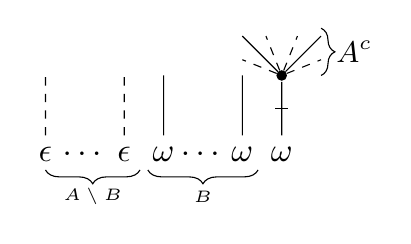
\begin{tikzpicture}
        \node (e1) at (-1.5,-.5) {$\epsilon$};
        \node at (-1,-.5) {$\dots$};
        \node (e2) at (-.5,-.5) {$\epsilon$};
        \node (w1) at (0,-.5) {$\omega$};
        \node at (0.5,-.5) {$\dots$};
        \node (w2) at (1,-.5) {$\omega$};
        \node (w_) at (1.5,-.5) {$\omega$};
        \node[int] (v) at (1.5,.5) {};
        \draw (e1) edge[dashed] +(0,1) (e2) edge[dashed] +(0,1);
        \draw (w1) edge +(0,1) (w2) edge +(0,1);
        \draw (w_) edge[crossed] (v);
        \draw (v) edge +(.5,.5)  edge[dashed] +(.5,.2) edge[dashed] +(.2,.5);
        \draw (v) edge +(-.5,.5) edge[dashed] +(-.5,.2) edge[dashed] +(-.2,.5);
        \draw [decorate,decoration={brace,mirror,amplitude=5pt}]
        (-1.5,-.7) -- (-.3,-.7) node[midway,yshift=-0.8em]{\tiny $A\setminus B$};
        \draw [decorate,decoration={brace,mirror,amplitude=5pt}]
        (-.2,-.7) -- (1.2,-.7) node[midway,yshift=-0.8em]{\tiny $B$};
        \draw [decorate,decoration={brace,mirror,amplitude=5pt}]
        (2,.5) -- (2,1.1) node[midway,xshift=1em]{\small $A^c$};
    \end{tikzpicture}
    \hspace{1cm}
\]
The crucial observation is that, if $C_1,..,C_k$ are the blown-up components of $G$, graph automorphisms $\phi:G\rightarrow G$ fixing $\bar{v}$ precisely correlate to permutations $\sigma\in\ss_k$ and graph isomorphisms $\phi_i:C_i\rightarrow C_{\sigma(i)}$. Thus, a generator $G$ is uniquely determined by its list of blown-up components up to reordering and isomorphism of the components preserving the features $\epsilon,\omega$, the original $n$ hairs and the crossed edge. In addition, a generator has an odd symmetry if and only if it has either a blown-up component with an odd symmetry (when restricted to internal edges and $\epsilon$ hairs, as the sign on $\omega$ cancels out by the action on the cohomology class) or at least two isomorphic blown-up components wich have an odd number of internal edges plus $\epsilon$ hairs (as the action on $\omega$ hairs cancels out).

This is already a concrete description that could be implemented in a computer algebra system. However, it would be very computationally wasteful to generate for each $(g,n)$ all isomorphism classes of $(g,n)$-stable graphs because the most efficient graph generating algorithms run based on the number of vertices.

Notice that the $(g,n)$ type of a graph $G$ can be be computed from the $(g,n)$ type and the number of $\epsilon$ and $\omega$ labels of each blown-up component. This means that we could first classify a set of blown-up components based on these parameters and afterwards generate all blown-up representations with these components. If we knew that the blow-up of every graph in some $(g,n)$ classes is so representable we would obtain the full $\bGK_{g,n}^{12,1}$ for multiple $(g,n)$ at a time, thus minimizing computational redundancy.

The authors of \cite[Section 3.2]{CLPW2} have chosen to classify blown-up representations by their excess value $E(g,n) = 3g+2n$, which fits together as follows with the parameters of blown-up components:
\[ n_{\bar{v}} = \sum_i\epsilon_i+\omega_i \geq 11 \hspace{1cm} n = \sum_i n_i \hspace{1cm} g = 1+\sum_i(g_i+\epsilon_i+\omega_i-1) \]
\[ 2(g-1)+n = n_{\bar{v}}+\sum_i 2(g_i-1)+\epsilon_i+\omega_i+n_i \hspace{1.5cm}  \forall i: 3(g_i-1)+3\epsilon_i+\omega_i+2n_i \geq 0\]
\[ 3(g-1)+2n = n_{\bar{v}}+\sum_i 3(g_i-1)+2(\epsilon_i+\omega_i+n_i) = 22+\sum_i 3(g_i-1)+3\epsilon_i+\omega_i+2n_i,
\]
where $g_i,\epsilon_i,\omega_i,n_i$ are the genus, number of $\epsilon$ labels, number of $\omega$ labels and number of original hairs of the $i$-th blown-up component. The excess is greater or equal to $25$ and additive over the non-negative paramenter $e(C_i)=3(g_i-1)+3\epsilon_i+\omega_i+2n_i$ of blown-up components, meaning that excess $E$ graphs can only be obtained from a list of blown-up components with $e$ summing up to $E-25$.

One reason for considering this function as a measure of complexity is its invariance under replacing three hairs at the special vertex by a 'tripod', meaning that in the excess classification we deal simultaneously with every combination of these two types of graphs, which are arguably the simplest stable subgraphs connected to the special vertex.
\[
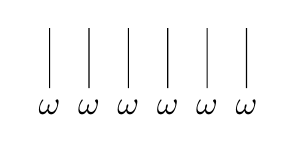
\begin{tikzpicture}
    \node (w1) at (0,-.5) {$\omega$};
    \node (w2) at (.5,-.5) {$\omega$};
    \node (w3) at (1,-.5) {$\omega$};
    \node (w4) at (1.5,-.5) {$\omega$};
    \node (w5) at (2,-.5) {$\omega$};
    \node (w6) at (2.5,-.5) {$\omega$};
    \draw (w1) edge +(0,1) (w2) edge +(0,1)  (w3) edge +(0,1)  (w4) edge +(0,1)  (w5) edge +(0,1)  (w6) edge +(0,1);
\end{tikzpicture}
,
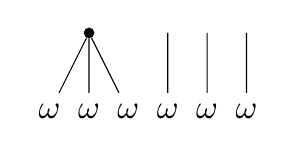
\begin{tikzpicture}
    \node[int] (v) at (.5,.5) {};
    \node (w1) at (0,-.5) {$\omega$};
    \node (w2) at (.5,-.5) {$\omega$};
    \node (w3) at (1,-.5) {$\omega$};
    \node (w4) at (1.5,-.5) {$\omega$};
    \node (w5) at (2,-.5) {$\omega$};
    \node (w6) at (2.5,-.5) {$\omega$};
    \draw (w1) edge (v) (w2) edge (v)  (w3) edge (v)  (w4) edge +(0,1)  (w5) edge +(0,1)  (w6) edge +(0,1);
\end{tikzpicture}
,
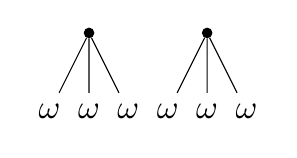
\begin{tikzpicture}
    \node[int] (v) at (.5,.5) {};
    \node[int] (v2) at (2,.5) {};
    \node (w1) at (0,-.5) {$\omega$};
    \node (w2) at (.5,-.5) {$\omega$};
    \node (w3) at (1,-.5) {$\omega$};
    \node (w4) at (1.5,-.5) {$\omega$};
    \node (w5) at (2,-.5) {$\omega$};
    \node (w6) at (2.5,-.5) {$\omega$};
    \draw (w1) edge (v) (w2) edge (v)  (w3) edge (v)  (w4) edge (v2)  (w5) edge (v2)  (w6) edge (v2);
\end{tikzpicture}
  \text{ \;\; all have $3(g-1)+2n=12$}
\]

\subsection{Action of the differential on the generators} \label{subsec:differential}
In the simplified graph complex $\bGK^{12,1}_{g,n}$, the differential $d$ acts by summing over every vertex and every way of splitting that vertex \cite[Section 2.6]{CLPW2}. More precisely, for every vertex $v$ of a decorated graph $(\Gamma,\gamma\otimes o)$, we consider the one-vertex decorated graph $(*_v,\gamma_v)$ whose hairs correspond to the hairs and neighbours of $v$ in $\Gamma$. The differential on one-vertex graphs decorated by the relevant cohomology classes is described in \ref{sec:1differential}. We denote by $d_v(\Gamma,\gamma\otimes o)$ the decorated graph obtained by replacing the vertex $v$ and it's decoration $\gamma_v$ by $d(*_{g,n},\gamma_v)$, gluing it's hairs to the hairs and neighbours of $v$ in $\Gamma$; the newly created edge is understood to be placed last in the alternating ordering $o$. Thus, the total differential takes the form


\[ \text{case (A): \;\;} (\Gamma,\gamma\otimes o) \xlongrightarrow{d} \hspace{.3cm} d_{\bar{v}}(\Gamma,\gamma\otimes o) \hspace{.1cm}  + \sum_{\bar{v}\neq v\in V(G)} d_v(\Gamma,\gamma\otimes o) \]
\[ \text{case (B): \;\;} (\Gamma,\gamma\otimes o) \xlongrightarrow{d} \hspace{.3cm} d_{\bar{v}}(\Gamma,\gamma\otimes o) \hspace{.1cm}  + d_{\tilde{v}}(\Gamma,\gamma\otimes o) +\sum_{\bar{v},\tilde{v}\neq v\in V(G)} d_v(\Gamma,\gamma\otimes o). \]



%\input{Low Excess Computations}
%\section{Computer Implementation}

\newpage
\section{Appendix} \label{sec:appendix}

The $\Q$-Hodge structure on the cohomology of the moduli space of curves delivers the following decompositions.
\begin{equation}\label{thm:GroupsHodgeDeco}
    H^{13}(\MM_{g,n})\otimes\CC = H^{12,1}(\MM_{g,n})\oplus H^{1,12}(\MM_{g,n})
\end{equation}
\[ H^{11}(\MM_{g,n})\otimes\CC = H^{11,0}(\MM_{g,n})\oplus H^{0,11}(\MM_{g,n}) \]
\[ H^{2}(\MM_{g,n})\otimes\CC = H^{1,1}(\MM_{g,n}) \]


In this paper we are interested in cohomology classes $\gamma_v\in H^k(\MM_{g,n})$ when viewed as decorations of a vertex of genus $g$ and valence $n$ in some graph $\Gamma$. Since it is cumbersome to bring along $\gamma$ whenever we want to reference a specific decorated graph $(\Gamma,\gamma)$, we will encode this datum in symbols drawn onto the vertex being decorated. The goal is to have graphical depictions that determine uniquely all relevant cohomology classes, so that just by the drawing it is possible to unambiguosly determine what is the decoration at each vertex. We will give these graphical depictions onto the one vertex graph $*_{g,n}$ of genus $g$ and with $n$ hairs, labeled by a set $N$; these depictions are understood to transfer onto the vertex being decorated of a general ambient graph.

To understand automorphisms of decorated graphs we will have to keep track of the $\ss_n$-action on each cohomolgy group induced by the permutation of $N$, which in some cases involves a sign representation.

In the following depictions, solid lines represent the minimum amount of edges \emph{necessary} for the considered class to exist, whereas dashed lines represent a \emph{potential} existance of edges.


\subsection{The case $k=0$, $g=0$, $n\geq 3$}

We have $H^{0,0}(\MM_{0,n})=\CC$ and thus we can draw weight $0$ vertices without any graphical depiction.
\[
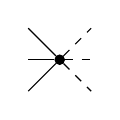
\begin{tikzpicture}
    \node[int] (v) at (0,0) {};
    \draw (v) edge[dashed] +(.4,0)  edge +(-.4,.4) edge[dashed] +(.4,.4);
    \draw (v) edge +(-.4,0) edge +(-.4,-.4)  edge[dashed] +(.4,-.4);
\end{tikzpicture}
:= (*_{0,n},1)
\]

\subsection{The case $k=(1,1)$, $g=1$,$n=1$}
$H^{1,1}(\MM_{1,1})$ is one dimensional, spanned the class we call $\delta_{irr}$. Since this is the only case where a non special vertex might have genus $1$, we will introduce a symbolic loop with a crossed edge and draw the node black as if it were a genus $0$ vertex. As $n=1$, there is no $\ss_n$-action on $\delta_irr$ to talk about.
\[
\begin{tikzpicture}
    \node[int] (v) at (0,0) {};
    \draw (v) edge +(0,-.3) edge[loop, crossed, distance=0.8cm] (v);
\end{tikzpicture}
:= (*_{1,1},\delta_{irr})
\]


\subsection{The case $k=(1,1)$, $g=0$} For this case we refer to \cite[Section 3]{PayneWillwacher21}.
In $g=0$, $H^{1,1}(\MM_{0,n})$ is non zero only for $n\geq 4$; so we operate under this assumption.
The group is generated by classes $\psi_i$ for every $1\leq i\leq n$ and $\delta\{\substack{A \\ A'}\}$ for every partition $A\sqcup A'=N$ with $|A|,|A'|\geq 2$. To depict $\delta\{\substack{A \\ A'}\}$ we split symbolically the vertex in two parts connected by a crossed edge and draw on one side the subset of hairs $A$ and on the other $A'$. The notation $\{\substack{A \\ A'}\}$ is chosen to express the fact that swapping $A$ and $A'$ doesn't change the class, which graphically means it doesn't matter on which sides the two sets of hairs are chosen to be drawn. The $\ss_n$-action is given by $\sigma\,\psi_i = \psi_{\sigma i}$ and $\sigma\,\delta\{\substack{A \\ A'}\}=\delta\{\substack{\sigma A \\ \sigma A'}\}$.

\[
    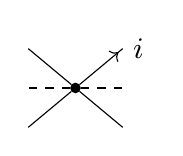
\begin{tikzpicture}
        \node[int] (v) at (0,0) {};
        \draw (v) edge[dashed] +(.6,0)  edge +(-.6,.5) edge[->-] +(.6,.5);
        \draw (v) edge[dashed] +(-.6,0) edge +(-.6,-.5)  edge +(.6,-.5);
        \node (x) at (.8,.5) {\small $i$};
    \end{tikzpicture}
    := (*_{0,n},\psi_i)
    \hspace{1cm}
    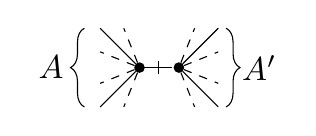
\begin{tikzpicture}
        \node[int] (v) at (0,0) {};
        \node[int] (w) at (0.5,0) {};
        \draw (v) edge +(-.5,-.5) edge +(-.5,.5) edge[dashed] +(-.5,.2) edge[dashed] +(-.2,.5) edge[dashed] +(-.5,-.2) edge[dashed] +(-.2,-.5) edge[crossed] (w)
        (w) edge +(.5,-.5) edge +(.5,.5) edge[dashed] +(.5,.2) edge[dashed] +(.5,-.2) edge[dashed] +(.2,.5) edge[dashed] +(.2,-.5);
        \draw [decorate,decoration={brace,amplitude=5pt,mirror}]
        (-.7,.5) -- (-.7,-.5) node[midway,xshift=-1em]{$A$};
        \draw [decorate,decoration={brace,amplitude=5pt}]
        (1.1,.5) -- (1.1,-.5) node[midway,xshift=1em]{$A'$};
    \end{tikzpicture}
    := (*_{0,n},\delta\{\substack{A \\ A'}\})
\]
There are two equivalent families of relations between these generators. For any three pairwise distinct $i,x,y\in N$, or for any $i\neq j\in N$, it holds: 
\begin{equation} \label{equ:Relations2}
    \psi_i = \sum_{\substack{A\sqcup A'=N,|A|,|A'|\geq 2 \\ i\in A,x,y\in A'}} \delta\{\substack{A \\ A'}\}  \hspace{2cm}  \psi_i+\psi_j = \sum_{\substack{A\sqcup A'=N,|A|,|A'|\geq 2 \\ i\in A,j\in A'}} \delta\{\substack{A \\ A'}\}.
\end{equation}
So the $\psi_i$ classes are actually superfluous in the case $g=0$, but algebraically they can be more convenient to work with. The dimension of $H^{1,1}(\MM_{0,n})$ turns out to be $2^{n-1}- \binom{n}{2} -1$, in particular when $n=4$ every single class forms a basis.

\subsection{The case $k=(11,0)$, $g=1$} This case is studied in \cite[Section 2]{CLP}. $H^{11,0}(\MM_{1,n})$ is non zero only for $n\geq 11$; so we operate under this assumption. The group is generated by classes $\omega_B$ for every \emph{alternatingly ordered} $B\subseteq N$ with $|B|=11$. This means that the underlying set determines $\omega_B$ up to sign, and if we choose a canonical labeling $N=\{1,...,n\}$ we can stipulate that every subset comes equipped with the increasing ordering. We draw arrows onto the hairs contained in $B$ to depict the $\omega_B$ decoration.
\[
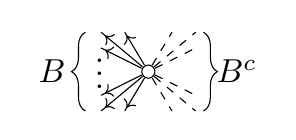
\begin{tikzpicture}
    \node[ext] (v) at (0,0) {};
    \node at (-.62, .1) {$\scriptscriptstyle \vdots$};
    \draw (v) edge[->-] +(-.6,-.5) edge[->-] +(-.6,-.3) edge[->-] +(-.3,-.5)
    edge[->-] +(-.6,.5) edge[->-] +(-.6,.3) edge[->-] +(-.3,.5) 
    edge[dashed] +(.6,.5) edge[dashed] +(.6,+.3)  edge[dashed] +(.3,+.5)
    edge[dashed] +(.6,-.5) edge[dashed] +(.6,-.3) edge[dashed] +(.3,-.5) ;
    \draw [decorate,decoration={brace,amplitude=5pt,mirror}]
  (-.8,.5) -- (-.8,-.5) node[midway,xshift=-1em]{$B$};
    \draw [decorate,decoration={brace,amplitude=5pt}]
    (.7,.5) -- (.7,-.5) node[midway,xshift=1em]{$B^c$};
\end{tikzpicture}
:= (*_{1,n},\omega_B)
\]

The only relations are amongst the classes $\omega_B$ whose set $B$ is contained in the same size $12$ subset. Namely, if we choose a canonical labeling on $N$, then for every $E=\{e_1,...,e_{12}\}\subseteq N$ with $e_i$ increasing there is the relation
\begin{equation} \label{equ:Relations11}
    \sum_{i=1}^{12} (-1)^i \omega_{E\setminus e_i} =0
\end{equation}
Therefore, choosing a distinguished hair $e\in N$ (for example $e=1$), the classes $\omega_B$ with $e\in B$ form a basis of $H^{11,0}(\MM_{1,n})$.

The $\ss_n$-action on $\omega_B$ is given by $\sigma\,\omega_B=\omega_{\sigma B}$, which is equal to $\sgn \sigma \,\omega_B$ if $\sigma$ preserves $B$ setwise.


\subsection{The case $k=(12,1)$, $g=1$} This case is studied in \cite[Section 4.2]{CLPW}.
$H^{12,1}(\MM_{1,n})$ is non zero only for $n\geq 12$; so we operate under this assumption. The group is generated by classes $Z_{B\subseteq A}$ for every subset $A\subseteq N$ with $|A^c|\geq 2$ and \emph{alternatingly ordered} subset $B\subseteq A$ with $|B|=10$; the underlying set $B$ determines $Z_{B\subseteq A}$ up to sign. We draw arrows onto the hairs contained in $B$, and we split symbolically the vertex in a genus $1$ vertex, where we attach the hairs in $A$, and a genus $0$ vertex, where we attach the hairs in $A^c$.

\[
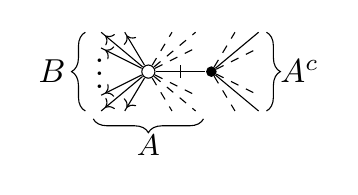
\begin{tikzpicture}
    \node[ext] (v) at (0,0) {};
    \node at (-.62, .1) {$\scriptscriptstyle \vdots$};
    \node[int] (w) at (.8, 0) {};
    \draw (v) edge[->-] +(-.6,-.5) edge[->-] +(-.6,-.3) edge[->-] +(-.3,-.5)
    edge[->-] +(-.6,.5) edge[->-] +(-.6,.3) edge[->-] +(-.3,.5) 
    edge[dashed] +(.6,.5) edge[dashed] +(.6,+.3)  edge[dashed] +(.3,+.5)
    edge[dashed] +(.6,-.5) edge[dashed] +(.6,-.3) edge[dashed] +(.3,-.5) edge[crossed] (w);
    \draw (w) edge +(.6,.5) edge[dashed] +(.6,+.3)  edge[dashed] +(.3,+.5)
    edge +(.6,-.5) edge[dashed] +(.6,-.3) edge[dashed] +(.3,-.5);
    \draw [decorate,decoration={brace,amplitude=5pt,mirror}]
    (-.8,.5) -- (-.8,-.5) node[midway,xshift=-1em]{$B$};
    \draw [decorate,decoration={brace,amplitude=5pt}]
    (1.5,.5) -- (1.5,-.5) node[midway,xshift=1em]{$A^c$};
    \draw [decorate,decoration={brace,mirror,amplitude=5pt}]
    (-.7,-.6) -- (.7,-.6) node[midway,yshift=-0.8em]{\small $A$};
\end{tikzpicture}
:= (*_{1,n},Z_{B\subseteq A})
\]

The only relations are amongst the classes $Z_{B\subseteq A}$ having $|A^c|=2$ and same set $B\sqcup A^c$. Namely, if we choose a canonical labeling on $N$, then for every $E=\{e_1,...,e_{12}\}\subseteq N$ with $e_i$ increasing and every $1\leq i<j<k\leq 12$ we have the relation
\begin{equation} \label{equ:Relations13}
    (-1)^{i+j}Z_{E\setminus e_i,e_j \subseteq N\setminus e_i,e_j} - (-1)^{i+k}Z_{E\setminus e_i,e_k\subseteq N\setminus e_i,e_k} + (-1)^{j+k}Z_{E\setminus e_j,e_k\subseteq N\setminus e_j,e_k} = 0
\end{equation}
For this subset $E\subseteq N$, choosing a distinguished element $e\in E$ (for example $e=e_1$), the subspace $PB_E$ spanned by the classes $Z_{B\subseteq A}$ with $B\sqcup A^c=E$ has basis the ones with $e\in A^c$, of which there are $11$. So $H^{12,1}(\MM_{1,n})$ decomposes into a direct sum $PB_3 \oplus \bigoplus_{|E|=12} PB_E$, where $PB_3$ has basis the classes with $|A^c|\geq 3$.
The $\ss_n$-action on $Z_{B\subseteq A}$ is given by $\sigma\,Z_{B\subseteq A}=Z_{\sigma B\subseteq \sigma A}$, which is equal to $\sgn \sigma \,Z_{B\subseteq \sigma A}$ if $\sigma$ preserves $B$ setwise.





\subsection{Action of the differential on cohomology classes} \label{sec:1differential}
In this section we describe the action of the differential operator that splits one-vertex decorated graphs.
A splitting of a decorated graph $(*_{g,n},\gamma)$ is of the form $(*'-*'',\gamma'\otimes\gamma'')$, where $*'-*''$ is the connection of two vertices $*'_{g',n'},*''_{g'',n''}$ with $g=g'+g''$, $n=n'+n''+2$, and $\gamma',\gamma''$ are their respective decorations.
The hairs of $*'$ and $*''$ form a partition of $N$. If $q'$ and $q''$ are the two half-edges connecting $*'$ and $*''$, then $\gamma'$ is obtained from $\gamma$ by pullback along the map $\MM_{g',n'+1}\rightarrow \MM_{g,n}$ determined by the subset of hairs ending up on $*'$. For the computation of the pullbacks of cohomology classes we refer to \cite{PayneWillwacher21},\cite{CLP} and \cite{CLPW} for the weight $2$, weight $11$ and weight $13$ cases respectively, in this paper we limit ourselves to translating those computations in graphical form.\\

The image under the differential is given by summing over these two-vertex decorated graphs for all possible splittings. In the case of interest, we always have either $g'=g''=g=0$ or $g'=g=1,g''=0$, so the only determining datum of the splitting is the partition of the hairs of $*_{g,n}$.
%In the terms where the alternatigly ordered subsets $B$ are modified in \ref{equ:Diff11} and \ref{equ:Diff12}, the half-edge $q$ is understood to take $\tilde{b}$s place in the ordering of $B$. In the two terms where a weight $11$ decoration is created out of a weight $13$ one, the half-edge $q$ is understood to be the last in the ordering of $B\sqcup q$.

\begin{equation} \label{equ:Diff1}
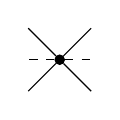
\begin{tikzpicture}
    \node[int] (v) at (0,0) {};
    \draw (v) edge[dashed] +(.4,0)  edge +(-.4,.4) edge +(.4,.4);
    \draw (v) edge[dashed] +(-.4,0) edge +(-.4,-.4)  edge +(.4,-.4);
\end{tikzpicture}
\hspace{.3in}
\xlongrightarrow{d}
\hspace{.3in}
\sum_{\substack{S\sqcup S' = N \\ |S|,|S'|\geq 2}}
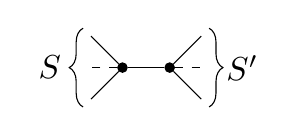
\begin{tikzpicture}
    \node[int] (v) at (0,0) {};
    \node[int] (w) at (.6,0) {};
    \draw (v) edge[dashed] +(-.4,0)  edge +(-.4,.4) edge +(-.4,-.4) edge (w);
    \draw (w) edge[dashed] +(.4,0) edge +(.4,.4)  edge +(.4,-.4);
    \draw [decorate,decoration={brace,amplitude=5pt,mirror}]
    (-.5,.5) -- (-.5,-.5) node[midway,xshift=-1em]{$S$};
    \draw [decorate,decoration={brace,amplitude=5pt}]
    (1.1,.5) -- (1.1,-.5) node[midway,xshift=1em]{$S'$};
\end{tikzpicture}
\end{equation}


\begin{equation} \label{equ:Diff2irr}
    \begin{tikzpicture}
        \node[int] (v) at (0,0) {};
        \draw (v) edge +(0,-.3) edge[loop, crossed, distance=0.8cm] (v);
    \end{tikzpicture}
\hspace{.1in}
\xlongrightarrow{d}
\hspace{.1in}
0 \hspace{.3in} \text{because the valence of $*_{1,1}$ is less than $2$}
\end{equation}


\begin{multline} \label{equ:Diff2}
\text{For any choice of $x,y\in A$ and $x',y'\in A'$, the image can be expressed as follows:}\\
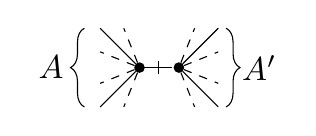
\begin{tikzpicture}
    \node[int] (v) at (0,0) {};
    \node[int] (w) at (0.5,0) {};
    \draw (v) edge +(-.5,-.5) edge +(-.5,.5) edge[dashed] +(-.5,.2) edge[dashed] +(-.2,.5) edge[dashed] +(-.5,-.2) edge[dashed] +(-.2,-.5) edge[crossed] (w)
    (w) edge +(.5,-.5) edge +(.5,.5) edge[dashed] +(.5,.2) edge[dashed] +(.5,-.2) edge[dashed] +(.2,.5) edge[dashed] +(.2,-.5);
    \draw [decorate,decoration={brace,amplitude=5pt,mirror}]
    (-.7,.5) -- (-.7,-.5) node[midway,xshift=-1em]{$A$};
    \draw [decorate,decoration={brace,amplitude=5pt}]
    (1.1,.5) -- (1.1,-.5) node[midway,xshift=1em]{$A'$};
\end{tikzpicture}
\hspace{.05in}
\xlongrightarrow{d}
\hspace{.05in}
-\sum_{x,y\in\tilde{A}\subset A}
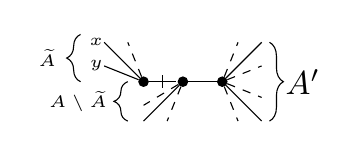
\begin{tikzpicture}
    \node[int] (v) at (0,0) {};
    \node[int] (w) at (0.5,0) {};
    \node[int] (z) at (1,0) {};
    \node[] (x) at (-.6,.5) {\tiny $x$};
    \node[] (y) at (-.6,.2) {\tiny $y$};
    \draw (v)  edge +(-.5,.5) edge +(-.5,.2) edge[dashed] +(-.2,.5)  edge[crossed] (w)
    (w) edge (z) edge +(-.5,-.5) edge[dashed] +(-.5,-.3) edge[dashed] +(-.2,-.5);
    \draw (z) edge +(.5,-.5) edge +(.5,.5) edge[dashed] +(.5,.2) edge[dashed] +(.5,-.2) edge[dashed] +(.2,.5) edge[dashed] +(.2,-.5);
    \draw [decorate,decoration={brace,amplitude=5pt,mirror}]
    (-.8,.6) -- (-.8,0) node[midway,xshift=-1em]{\tiny $\tilde{A}$};
    \draw [decorate,decoration={brace,amplitude=5pt,mirror}]
    (-.2,0) -- (-.2,-.5) node[midway,xshift=-1.5em]{\tiny $A\setminus\tilde{A}$};
    \draw [decorate,decoration={brace,amplitude=5pt}]
    (1.6,.5) -- (1.6,-.5) node[midway,xshift=1em]{$A'$};
\end{tikzpicture}
-\sum_{x',y'\in\tilde{A}\subset A'}
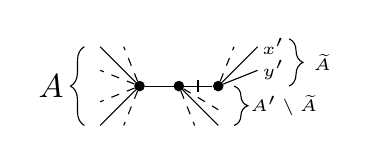
\begin{tikzpicture}
    \node[int] (z) at (-1,0) {};
    \node[int] (v) at (-0.5,0) {};
    \node[int] (w) at (0,0) {};
    \node[] (x) at (.7,.5) {\tiny $x'$};
    \node[] (y) at (.7,.2) {\tiny $y'$};
    \draw (z) edge +(-.5,-.5) edge +(-.5,.5) edge[dashed] +(-.5,.2) edge[dashed] +(-.2,.5) edge[dashed] +(-.5,-.2) edge[dashed] +(-.2,-.5) edge (v);
    \draw (v) edge[crossed] (w) edge +(.5,-.5) edge[dashed] +(.5,-.3) edge[dashed] +(.2,-.5);
    \draw (w) edge +(.5,.5) edge +(.5,.2) edge[dashed] +(.2,.5) ;
    \draw [decorate,decoration={brace,amplitude=5pt,mirror}]
    (-1.7,.5) -- (-1.7,-.5) node[midway,xshift=-1em]{$A$};
    \draw [decorate,decoration={brace,amplitude=5pt}]
    (.9,.6) -- (.9,0) node[midway,xshift=1em]{\tiny $\tilde{A}$};
    \draw [decorate,decoration={brace,amplitude=5pt}]
    (.2,0) -- (.2,-.5) node[midway,xshift=1.5em]{\tiny $A'\setminus\tilde{A}$};
\end{tikzpicture}\\
+\sum_{\substack{S\subset A' \\ |S|\geq 2}}
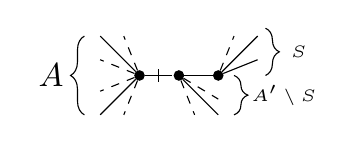
\begin{tikzpicture}
    \node[int] (z) at (-1,0) {};
    \node[int] (v) at (-0.5,0) {};
    \node[int] (w) at (0,0) {};
    \draw (z) edge +(-.5,-.5) edge +(-.5,.5) edge[dashed] +(-.5,.2) edge[dashed] +(-.2,.5) edge[dashed] +(-.5,-.2) edge[dashed] +(-.2,-.5) edge[crossed] (v);
    \draw (v) edge (w) edge +(.5,-.5) edge[dashed] +(.5,-.3) edge[dashed] +(.2,-.5);
    \draw (w) edge +(.5,.5) edge +(.5,.2) edge[dashed] +(.2,.5) ;
    \draw [decorate,decoration={brace,amplitude=5pt,mirror}]
    (-1.7,.5) -- (-1.7,-.5) node[midway,xshift=-1em]{$A$};
    \draw [decorate,decoration={brace,amplitude=5pt}]
    (.6,.6) -- (.6,0) node[midway,xshift=1em]{\tiny $S$};
    \draw [decorate,decoration={brace,amplitude=5pt}]
    (.2,0) -- (.2,-.5) node[midway,xshift=1.5em]{\tiny $A'\setminus S$};
\end{tikzpicture}
+\sum_{\substack{S\subset A \\ |S|\geq 2}}
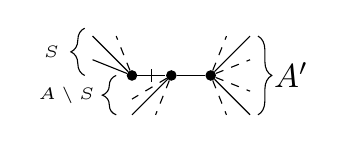
\begin{tikzpicture}
    \node[int] (v) at (0,0) {};
    \node[int] (w) at (0.5,0) {};
    \node[int] (z) at (1,0) {};
    \draw (v)  edge +(-.5,.5) edge +(-.5,.2) edge[dashed] +(-.2,.5)  edge[crossed] (w)
    (w) edge (z) edge +(-.5,-.5) edge[dashed] +(-.5,-.3) edge[dashed] +(-.2,-.5);
    \draw (z) edge +(.5,-.5) edge +(.5,.5) edge[dashed] +(.5,.2) edge[dashed] +(.5,-.2) edge[dashed] +(.2,.5) edge[dashed] +(.2,-.5);
    \draw [decorate,decoration={brace,amplitude=5pt,mirror}]
    (-.6,.6) -- (-.6,0) node[midway,xshift=-1em]{\tiny $S$};
    \draw [decorate,decoration={brace,amplitude=5pt,mirror}]
    (-.2,0) -- (-.2,-.5) node[midway,xshift=-1.5em]{\tiny $A\setminus S$};
    \draw [decorate,decoration={brace,amplitude=5pt}]
    (1.6,.5) -- (1.6,-.5) node[midway,xshift=1em]{$A'$};
\end{tikzpicture}
\end{multline}


In the second term, the weight $11$ decoration $\omega_B$ becomes $\omega_{B\setminus\tilde{b}\sqcup q}$, where $q$ is the newly added half-edge to the genus $1$ vertex and takes the place of $\tilde{b}$ in the ordering of $B$.
\begin{equation} \label{equ:Diff11}
    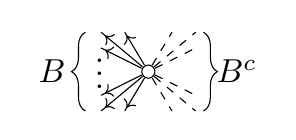
\begin{tikzpicture}
        \node[ext] (v) at (0,0) {};
        \node at (-.62, .1) {$\scriptscriptstyle \vdots$};
        \draw (v) edge[->-] +(-.6,-.5) edge[->-] +(-.6,-.3) edge[->-] +(-.3,-.5)
        edge[->-] +(-.6,.5) edge[->-] +(-.6,.3) edge[->-] +(-.3,.5) 
        edge[dashed] +(.6,.5) edge[dashed] +(.6,+.3)  edge[dashed] +(.3,+.5)
        edge[dashed] +(.6,-.5) edge[dashed] +(.6,-.3) edge[dashed] +(.3,-.5) ;
        \draw [decorate,decoration={brace,amplitude=5pt,mirror}]
      (-.8,.5) -- (-.8,-.5) node[midway,xshift=-1em]{$B$};
        \draw [decorate,decoration={brace,amplitude=5pt}]
        (.7,.5) -- (.7,-.5) node[midway,xshift=1em]{$B^c$};
    \end{tikzpicture}
    \hspace{.05in}
    \xlongrightarrow{d}
    \hspace{.05in}
    \sum_{\substack{S\subseteq B^c \\ |S|\geq 2}}
    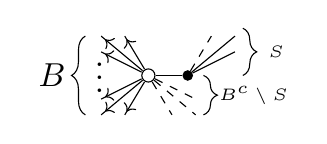
\begin{tikzpicture}
        \node[ext] (v) at (0,0) {};
        \node at (-.62, .1) {$\scriptscriptstyle \vdots$};
        \node[int] (z) at (.5,0) {};
        \draw (v) edge[->-] +(-.6,-.5) edge[->-] +(-.6,-.3) edge[->-] +(-.3,-.5)
        edge[->-] +(-.6,.5) edge[->-] +(-.6,.3) edge[->-] +(-.3,.5) 
        edge[dashed] +(.6,-.5) edge[dashed] +(.6,-.3) edge[dashed] +(.3,-.5) edge (z);
        \draw (z) edge +(.6,.5) edge +(.6,+.3)  edge[dashed] +(.3,+.5);
        \draw [decorate,decoration={brace,amplitude=5pt,mirror}]
      (-.8,.5) -- (-.8,-.5) node[midway,xshift=-1em]{$B$};
        \draw [decorate,decoration={brace,amplitude=5pt}]
        (1.2,.6) -- (1.2,0) node[midway,xshift=1em]{\tiny $S$};
        \draw [decorate,decoration={brace,amplitude=5pt}]
        (.7,0) -- (.7,-.5) node[midway,xshift=1.5em]{\tiny $B^c\setminus S$};
    \end{tikzpicture}
    +\sum_{\substack{\varnothing\neq S\subseteq B^c \\ \tilde{b}\in B}}
    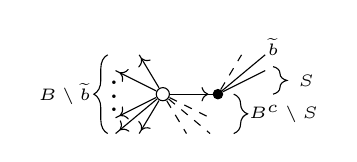
\begin{tikzpicture}
        \node[ext] (v) at (0,0) {};
        \node at (-.62, .1) {$\scriptscriptstyle \vdots$};
        \node[int] (z) at (.7,0) {};
        \node (b) at (1.4,.6) {\tiny $\tilde{b}$};
        \draw (v) edge[->-] +(-.6,-.3) edge[->-] +(-.6,-.5) edge[->-] +(-.3,-.5)
        edge[->-] +(-.6,.3) edge[->-] +(-.3,.5) 
        edge[dashed] +(.6,-.5) edge[dashed] +(.6,-.3) edge[dashed] +(.3,-.5) edge[->-] (z);
        \draw (z) edge +(.6,.5) edge +(.6,+.3)  edge[dashed] +(.3,+.5);
        \draw [decorate,decoration={brace,amplitude=5pt,mirror}]
      (-.7,.5) -- (-.7,-.5) node[midway,xshift=-1.3em]{\tiny $B\setminus\tilde{b}$};
        \draw [decorate,decoration={brace,amplitude=5pt}]
        (1.4,.35) -- (1.4,0) node[midway,xshift=1em]{\tiny $S$};
        \draw [decorate,decoration={brace,amplitude=5pt}]
        (.9,0) -- (.9,-.5) node[midway,xshift=1.5em]{\tiny $B^c\setminus S$};
    \end{tikzpicture}
\end{equation}


For any fixed choice of $x,y\in A^c$, the image can be expressed as in \ref{equ:Diff12}. In the two terms that create weight $11$ and $2$ vertices, the newly created weight $11$ decoration $\omega_{B\sqcup p}$, where $p$ is the half-edge at the genus $1$ vertex, is understood to have the ordering inherited from $B$ with $p$ appended at the end.
\begin{multline}\label{equ:Diff12}  
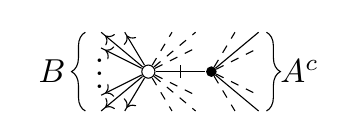
\begin{tikzpicture}
    \node[ext] (v) at (0,0) {};
    \node at (-.62, .1) {$\scriptscriptstyle \vdots$};
    \node[int] (w) at (.8, 0) {};
    \draw (v) edge[->-] +(-.6,-.5) edge[->-] +(-.6,-.3) edge[->-] +(-.3,-.5)
    edge[->-] +(-.6,.5) edge[->-] +(-.6,.3) edge[->-] +(-.3,.5) 
    edge[dashed] +(.6,.5) edge[dashed] +(.6,+.3)  edge[dashed] +(.3,+.5)
    edge[dashed] +(.6,-.5) edge[dashed] +(.6,-.3) edge[dashed] +(.3,-.5) edge[crossed] (w);
    \draw (w) edge +(.6,.5) edge[dashed] +(.6,+.3)  edge[dashed] +(.3,+.5)
    edge +(.6,-.5) edge[dashed] +(.6,-.3) edge[dashed] +(.3,-.5);
    \draw [decorate,decoration={brace,amplitude=5pt,mirror}]
    (-.8,.5) -- (-.8,-.5) node[midway,xshift=-1em]{$B$};
    \draw [decorate,decoration={brace,amplitude=5pt}]
    (1.5,.5) -- (1.5,-.5) node[midway,xshift=1em]{$A^c$};
\end{tikzpicture}
\hspace{.05in}
\xlongrightarrow{d}
\hspace{.05in}
\sum_{\substack{S\subset A^c \\ |S|\geq 2}}
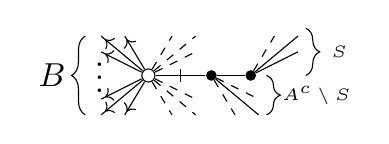
\begin{tikzpicture}
    \node[ext] (v) at (0,0) {};
    \node at (-.62, .1) {$\scriptscriptstyle \vdots$};
    \node[int] (w) at (.8, 0) {};
    \node[int] (z) at (1.3,0) {};
    \draw (v) edge[->-] +(-.6,-.5) edge[->-] +(-.6,-.3) edge[->-] +(-.3,-.5)
    edge[->-] +(-.6,.5) edge[->-] +(-.6,.3) edge[->-] +(-.3,.5) 
    edge[dashed] +(.6,.5) edge[dashed] +(.6,+.3)  edge[dashed] +(.3,+.5)
    edge[dashed] +(.6,-.5) edge[dashed] +(.6,-.3) edge[dashed] +(.3,-.5) edge[crossed] (w);
    \draw (w) edge +(.6,-.5) edge[dashed] +(.6,-.3) edge[dashed] +(.3,-.5) edge (z);
    \draw (z) edge +(.6,.5) edge +(.6,+.3)  edge[dashed] +(.3,+.5);
    \draw [decorate,decoration={brace,amplitude=5pt,mirror}]
    (-.8,.5) -- (-.8,-.5) node[midway,xshift=-1em]{$B$};
    \draw [decorate,decoration={brace,amplitude=5pt}]
    (2,.6) -- (2,0) node[midway,xshift=1em]{\tiny $S$};
    \draw [decorate,decoration={brace,amplitude=5pt}]
    (1.5,0) -- (1.5,-.5) node[midway,xshift=1.5em]{\tiny $A^c\setminus S$};
\end{tikzpicture}
+\sum_{\substack{\tilde{S}\subseteq A\setminus B \\ |\tilde{S}|\geq 2}}
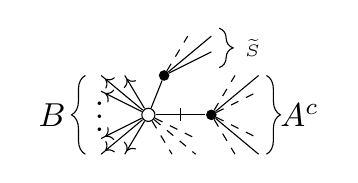
\begin{tikzpicture}
    \node[ext] (v) at (0,0) {};
    \node at (-.62, .1) {$\scriptscriptstyle \vdots$};
    \node[int] (w) at (.8, 0) {};
    \node[int] (z) at (.2,.5) {};
    \draw (v) edge (z) edge[->-] +(-.6,-.5) edge[->-] +(-.6,-.3) edge[->-] +(-.3,-.5)
    edge[->-] +(-.6,.5) edge[->-] +(-.6,.3) edge[->-] +(-.3,.5) 
    edge[dashed] +(.6,-.5) edge[dashed] +(.6,-.3) edge[dashed] +(.3,-.5) edge[crossed] (w);
    \draw (z) edge +(.6,.5) edge +(.6,+.3)  edge[dashed] +(.3,+.5);
    \draw (w) edge +(.6,.5) edge[dashed] +(.6,+.3)  edge[dashed] +(.3,+.5)
    edge +(.6,-.5) edge[dashed] +(.6,-.3) edge[dashed] +(.3,-.5);
    \draw [decorate,decoration={brace,amplitude=5pt,mirror}]
    (-.8,.5) -- (-.8,-.5) node[midway,xshift=-1em]{$B$};
    \draw [decorate,decoration={brace,amplitude=5pt}]
    (.9,1.1) -- (.9,.6) node[midway,xshift=1em]{\tiny $\tilde{S}$};
    \draw [decorate,decoration={brace,amplitude=5pt}]
    (1.5,.5) -- (1.5,-.5) node[midway,xshift=1em]{$A^c$};
\end{tikzpicture}\\
+\sum_{\substack{\varnothing\neq\tilde{S}\subseteq A\setminus B \\ \tilde{b}\in B}}
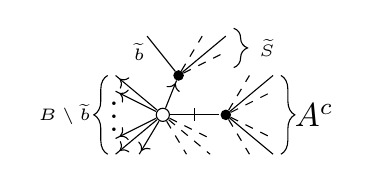
\begin{tikzpicture}
    \node[ext] (v) at (0,0) {};
    \node at (-.62, .1) {$\scriptscriptstyle \vdots$};
    \node[int] (w) at (.8, 0) {};
    \node[int] (z) at (.2,.5) {};
    \node (b) at (-.3,.8) {\tiny $\tilde{b}$};
    \draw (v) edge[->-] (z) edge[->-] +(-.6,-.5) edge[->-] +(-.6,-.3) edge[->-] +(-.3,-.5)
    edge[->-] +(-.6,.5) edge[->-] +(-.6,.3)
    edge[dashed] +(.6,-.5) edge[dashed] +(.6,-.3) edge[dashed] +(.3,-.5) edge[crossed] (w);
    \draw (z) edge +(.6,.5) edge[dashed] +(.6,+.3)  edge[dashed] +(.3,+.5) edge +(-.4,.5);
    \draw (w) edge +(.6,.5) edge[dashed] +(.6,+.3)  edge[dashed] +(.3,+.5)
    edge +(.6,-.5) edge[dashed] +(.6,-.3) edge[dashed] +(.3,-.5);
    \draw [decorate,decoration={brace,amplitude=5pt,mirror}]
    (-.7,.5) -- (-.7,-.5) node[midway,xshift=-1.3em]{\tiny$B\setminus\tilde{b}$};
    \draw [decorate,decoration={brace,amplitude=5pt}]
    (.9,1.1) -- (.9,.6) node[midway,xshift=1em]{\tiny $\tilde{S}$};
    \draw [decorate,decoration={brace,amplitude=5pt}]
    (1.5,.5) -- (1.5,-.5) node[midway,xshift=1em]{$A^c$};
\end{tikzpicture}
+\sum_{\varnothing\neq\tilde{S}\subseteq A\setminus B}
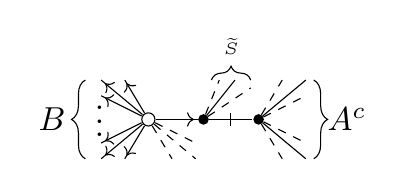
\begin{tikzpicture}
    \node[ext] (v) at (0,0) {};
    \node at (-.62, .1) {$\scriptscriptstyle \vdots$};
    \node[int] (w) at (.7, 0) {};
    \node[int] (z) at (1.4,0) {};
    \draw (v) edge[->-] +(-.6,-.5) edge[->-] +(-.6,-.3) edge[->-] +(-.3,-.5)
    edge[->-] +(-.6,.5) edge[->-] +(-.6,.3) edge[->-] +(-.3,.5) 
    edge[dashed] +(.6,-.5) edge[dashed] +(.6,-.3) edge[dashed] +(.3,-.5) edge[->-] (w);
    \draw (w)  edge[crossed] (z) edge +(.4,.5) edge[dashed] +(.6,+.4)  edge[dashed] +(.2,+.5);
    \draw (z) edge +(.6,.5) edge[dashed] +(.6,+.3)  edge[dashed] +(.3,+.5)
    edge +(.6,-.5) edge[dashed] +(.6,-.3) edge[dashed] +(.3,-.5);
    \draw [decorate,decoration={brace,amplitude=5pt,mirror}]
    (-.8,.5) -- (-.8,-.5) node[midway,xshift=-1em]{$B$};
    \draw [decorate,decoration={brace,amplitude=5pt}]
    (2.1,.5) -- (2.1,-.5) node[midway,xshift=1em]{$A^c$};
    \draw [decorate,decoration={brace,amplitude=5pt}]
    (.8,.5) -- (1.3,.5) node[midway,yshift=1em]{\tiny $\tilde{S}$};
\end{tikzpicture}\\
-\sum_{\varnothing\neq\tilde{S}\subseteq A\setminus B}
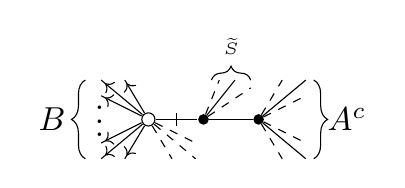
\begin{tikzpicture}
    \node[ext] (v) at (0,0) {};
    \node at (-.62, .1) {$\scriptscriptstyle \vdots$};
    \node[int] (w) at (.7, 0) {};
    \node[int] (z) at (1.4,0) {};
    \draw (v) edge[->-] +(-.6,-.5) edge[->-] +(-.6,-.3) edge[->-] +(-.3,-.5)
    edge[->-] +(-.6,.5) edge[->-] +(-.6,.3) edge[->-] +(-.3,.5) 
    edge[dashed] +(.6,-.5) edge[dashed] +(.6,-.3) edge[dashed] +(.3,-.5) edge[crossed] (w);
    \draw (w)  edge (z) edge +(.4,.5) edge[dashed] +(.6,+.4)  edge[dashed] +(.2,+.5);
    \draw (z) edge +(.6,.5) edge[dashed] +(.6,+.3)  edge[dashed] +(.3,+.5)
    edge +(.6,-.5) edge[dashed] +(.6,-.3) edge[dashed] +(.3,-.5);
    \draw [decorate,decoration={brace,amplitude=5pt,mirror}]
    (-.8,.5) -- (-.8,-.5) node[midway,xshift=-1em]{$B$};
    \draw [decorate,decoration={brace,amplitude=5pt}]
    (2.1,.5) -- (2.1,-.5) node[midway,xshift=1em]{$A^c$};
    \draw [decorate,decoration={brace,amplitude=5pt}]
    (.8,.5) -- (1.3,.5) node[midway,yshift=1em]{\tiny $\tilde{S}$};
\end{tikzpicture}
-\sum_{x,y\in S\subset A^c}
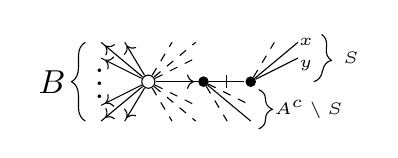
\begin{tikzpicture}
    \node[ext] (v) at (0,0) {};
    \node at (-.62, .1) {$\scriptscriptstyle \vdots$};
    \node[int] (w) at (.7, 0) {};
    \node[int] (z) at (1.3,0) {};
    \node (x) at (2,.5) {\tiny $x$};
    \node (y) at (2,.2) {\tiny $y$};
    \draw (v) edge[->-] +(-.6,-.5) edge[->-] +(-.6,-.3) edge[->-] +(-.3,-.5)
    edge[->-] +(-.6,.5) edge[->-] +(-.6,.3) edge[->-] +(-.3,.5) 
    edge[dashed] +(.6,.5) edge[dashed] +(.6,+.3)  edge[dashed] +(.3,+.5)
    edge[dashed] +(.6,-.5) edge[dashed] +(.6,-.3) edge[dashed] +(.3,-.5) edge[->-] (w);
    \draw (w) edge +(.6,-.5) edge[dashed] +(.6,-.3) edge[dashed] +(.3,-.5) edge[crossed] (z);
    \draw (z) edge +(.6,.5) edge +(.6,+.3)  edge[dashed] +(.3,+.5);
    \draw [decorate,decoration={brace,amplitude=5pt,mirror}]
    (-.8,.5) -- (-.8,-.5) node[midway,xshift=-1em]{$B$};
    \draw [decorate,decoration={brace,amplitude=5pt}]
    (2.2,.6) -- (2.1,0) node[midway,xshift=1em]{\tiny $S$};
    \draw [decorate,decoration={brace,amplitude=5pt}]
    (1.4,-.1) -- (1.4,-.6) node[midway,xshift=1.5em]{\tiny $A^c\setminus S$};
\end{tikzpicture}
\end{multline}




\bibliographystyle{amsplain}
\bibliography{refs}
\end{document}
